% Options for packages loaded elsewhere
% Options for packages loaded elsewhere
\PassOptionsToPackage{unicode}{hyperref}
\PassOptionsToPackage{hyphens}{url}
\PassOptionsToPackage{dvipsnames,svgnames,x11names}{xcolor}
%
\documentclass[
  letterpaper,
  DIV=11,
  numbers=noendperiod]{scrreprt}
\usepackage{xcolor}
\usepackage{amsmath,amssymb}
\setcounter{secnumdepth}{5}
\usepackage{iftex}
\ifPDFTeX
  \usepackage[T1]{fontenc}
  \usepackage[utf8]{inputenc}
  \usepackage{textcomp} % provide euro and other symbols
\else % if luatex or xetex
  \usepackage{unicode-math} % this also loads fontspec
  \defaultfontfeatures{Scale=MatchLowercase}
  \defaultfontfeatures[\rmfamily]{Ligatures=TeX,Scale=1}
\fi
\usepackage{lmodern}
\ifPDFTeX\else
  % xetex/luatex font selection
\fi
% Use upquote if available, for straight quotes in verbatim environments
\IfFileExists{upquote.sty}{\usepackage{upquote}}{}
\IfFileExists{microtype.sty}{% use microtype if available
  \usepackage[]{microtype}
  \UseMicrotypeSet[protrusion]{basicmath} % disable protrusion for tt fonts
}{}
\makeatletter
\@ifundefined{KOMAClassName}{% if non-KOMA class
  \IfFileExists{parskip.sty}{%
    \usepackage{parskip}
  }{% else
    \setlength{\parindent}{0pt}
    \setlength{\parskip}{6pt plus 2pt minus 1pt}}
}{% if KOMA class
  \KOMAoptions{parskip=half}}
\makeatother
% Make \paragraph and \subparagraph free-standing
\makeatletter
\ifx\paragraph\undefined\else
  \let\oldparagraph\paragraph
  \renewcommand{\paragraph}{
    \@ifstar
      \xxxParagraphStar
      \xxxParagraphNoStar
  }
  \newcommand{\xxxParagraphStar}[1]{\oldparagraph*{#1}\mbox{}}
  \newcommand{\xxxParagraphNoStar}[1]{\oldparagraph{#1}\mbox{}}
\fi
\ifx\subparagraph\undefined\else
  \let\oldsubparagraph\subparagraph
  \renewcommand{\subparagraph}{
    \@ifstar
      \xxxSubParagraphStar
      \xxxSubParagraphNoStar
  }
  \newcommand{\xxxSubParagraphStar}[1]{\oldsubparagraph*{#1}\mbox{}}
  \newcommand{\xxxSubParagraphNoStar}[1]{\oldsubparagraph{#1}\mbox{}}
\fi
\makeatother


\usepackage{longtable,booktabs,array}
\usepackage{calc} % for calculating minipage widths
% Correct order of tables after \paragraph or \subparagraph
\usepackage{etoolbox}
\makeatletter
\patchcmd\longtable{\par}{\if@noskipsec\mbox{}\fi\par}{}{}
\makeatother
% Allow footnotes in longtable head/foot
\IfFileExists{footnotehyper.sty}{\usepackage{footnotehyper}}{\usepackage{footnote}}
\makesavenoteenv{longtable}
\usepackage{graphicx}
\makeatletter
\newsavebox\pandoc@box
\newcommand*\pandocbounded[1]{% scales image to fit in text height/width
  \sbox\pandoc@box{#1}%
  \Gscale@div\@tempa{\textheight}{\dimexpr\ht\pandoc@box+\dp\pandoc@box\relax}%
  \Gscale@div\@tempb{\linewidth}{\wd\pandoc@box}%
  \ifdim\@tempb\p@<\@tempa\p@\let\@tempa\@tempb\fi% select the smaller of both
  \ifdim\@tempa\p@<\p@\scalebox{\@tempa}{\usebox\pandoc@box}%
  \else\usebox{\pandoc@box}%
  \fi%
}
% Set default figure placement to htbp
\def\fps@figure{htbp}
\makeatother


% definitions for citeproc citations
\NewDocumentCommand\citeproctext{}{}
\NewDocumentCommand\citeproc{mm}{%
  \begingroup\def\citeproctext{#2}\cite{#1}\endgroup}
\makeatletter
 % allow citations to break across lines
 \let\@cite@ofmt\@firstofone
 % avoid brackets around text for \cite:
 \def\@biblabel#1{}
 \def\@cite#1#2{{#1\if@tempswa , #2\fi}}
\makeatother
\newlength{\cslhangindent}
\setlength{\cslhangindent}{1.5em}
\newlength{\csllabelwidth}
\setlength{\csllabelwidth}{3em}
\newenvironment{CSLReferences}[2] % #1 hanging-indent, #2 entry-spacing
 {\begin{list}{}{%
  \setlength{\itemindent}{0pt}
  \setlength{\leftmargin}{0pt}
  \setlength{\parsep}{0pt}
  % turn on hanging indent if param 1 is 1
  \ifodd #1
   \setlength{\leftmargin}{\cslhangindent}
   \setlength{\itemindent}{-1\cslhangindent}
  \fi
  % set entry spacing
  \setlength{\itemsep}{#2\baselineskip}}}
 {\end{list}}
\usepackage{calc}
\newcommand{\CSLBlock}[1]{\hfill\break\parbox[t]{\linewidth}{\strut\ignorespaces#1\strut}}
\newcommand{\CSLLeftMargin}[1]{\parbox[t]{\csllabelwidth}{\strut#1\strut}}
\newcommand{\CSLRightInline}[1]{\parbox[t]{\linewidth - \csllabelwidth}{\strut#1\strut}}
\newcommand{\CSLIndent}[1]{\hspace{\cslhangindent}#1}



\setlength{\emergencystretch}{3em} % prevent overfull lines

\providecommand{\tightlist}{%
  \setlength{\itemsep}{0pt}\setlength{\parskip}{0pt}}



 


\KOMAoption{captions}{tableheading}
\makeatletter
\@ifpackageloaded{bookmark}{}{\usepackage{bookmark}}
\makeatother
\makeatletter
\@ifpackageloaded{caption}{}{\usepackage{caption}}
\AtBeginDocument{%
\ifdefined\contentsname
  \renewcommand*\contentsname{Table of contents}
\else
  \newcommand\contentsname{Table of contents}
\fi
\ifdefined\listfigurename
  \renewcommand*\listfigurename{List of Figures}
\else
  \newcommand\listfigurename{List of Figures}
\fi
\ifdefined\listtablename
  \renewcommand*\listtablename{List of Tables}
\else
  \newcommand\listtablename{List of Tables}
\fi
\ifdefined\figurename
  \renewcommand*\figurename{Figure}
\else
  \newcommand\figurename{Figure}
\fi
\ifdefined\tablename
  \renewcommand*\tablename{Table}
\else
  \newcommand\tablename{Table}
\fi
}
\@ifpackageloaded{float}{}{\usepackage{float}}
\floatstyle{ruled}
\@ifundefined{c@chapter}{\newfloat{codelisting}{h}{lop}}{\newfloat{codelisting}{h}{lop}[chapter]}
\floatname{codelisting}{Listing}
\newcommand*\listoflistings{\listof{codelisting}{List of Listings}}
\makeatother
\makeatletter
\makeatother
\makeatletter
\@ifpackageloaded{caption}{}{\usepackage{caption}}
\@ifpackageloaded{subcaption}{}{\usepackage{subcaption}}
\makeatother
\usepackage{bookmark}
\IfFileExists{xurl.sty}{\usepackage{xurl}}{} % add URL line breaks if available
\urlstyle{same}
\hypersetup{
  pdftitle={RMweekly},
  pdfauthor={Tianyi Chen},
  colorlinks=true,
  linkcolor={blue},
  filecolor={Maroon},
  citecolor={Blue},
  urlcolor={Blue},
  pdfcreator={LaTeX via pandoc}}


\title{RMweekly}
\author{Tianyi Chen}
\date{2026-03-27}
\begin{document}
\maketitle

\renewcommand*\contentsname{Table of contents}
{
\hypersetup{linkcolor=}
\setcounter{tocdepth}{2}
\tableofcontents
}

\bookmarksetup{startatroot}

\chapter*{Introduction}\label{introduction}
\addcontentsline{toc}{chapter}{Introduction}

\markboth{Introduction}{Introduction}

\section*{About me}\label{about-me}
\addcontentsline{toc}{section}{About me}

\markright{About me}

\textbf{Welcome to my remote sensing hub!} I'm Tianyi Chen, an MSc Urban
Spatial Science student at UCL. This digital space is dedicated to
documenting my journey through the CASA0023 module. Whether I'm trying
to make sense of spatial algorithms or just exploring the city, I'm
always looking for new ways to understand our urban environments.

\begin{center}
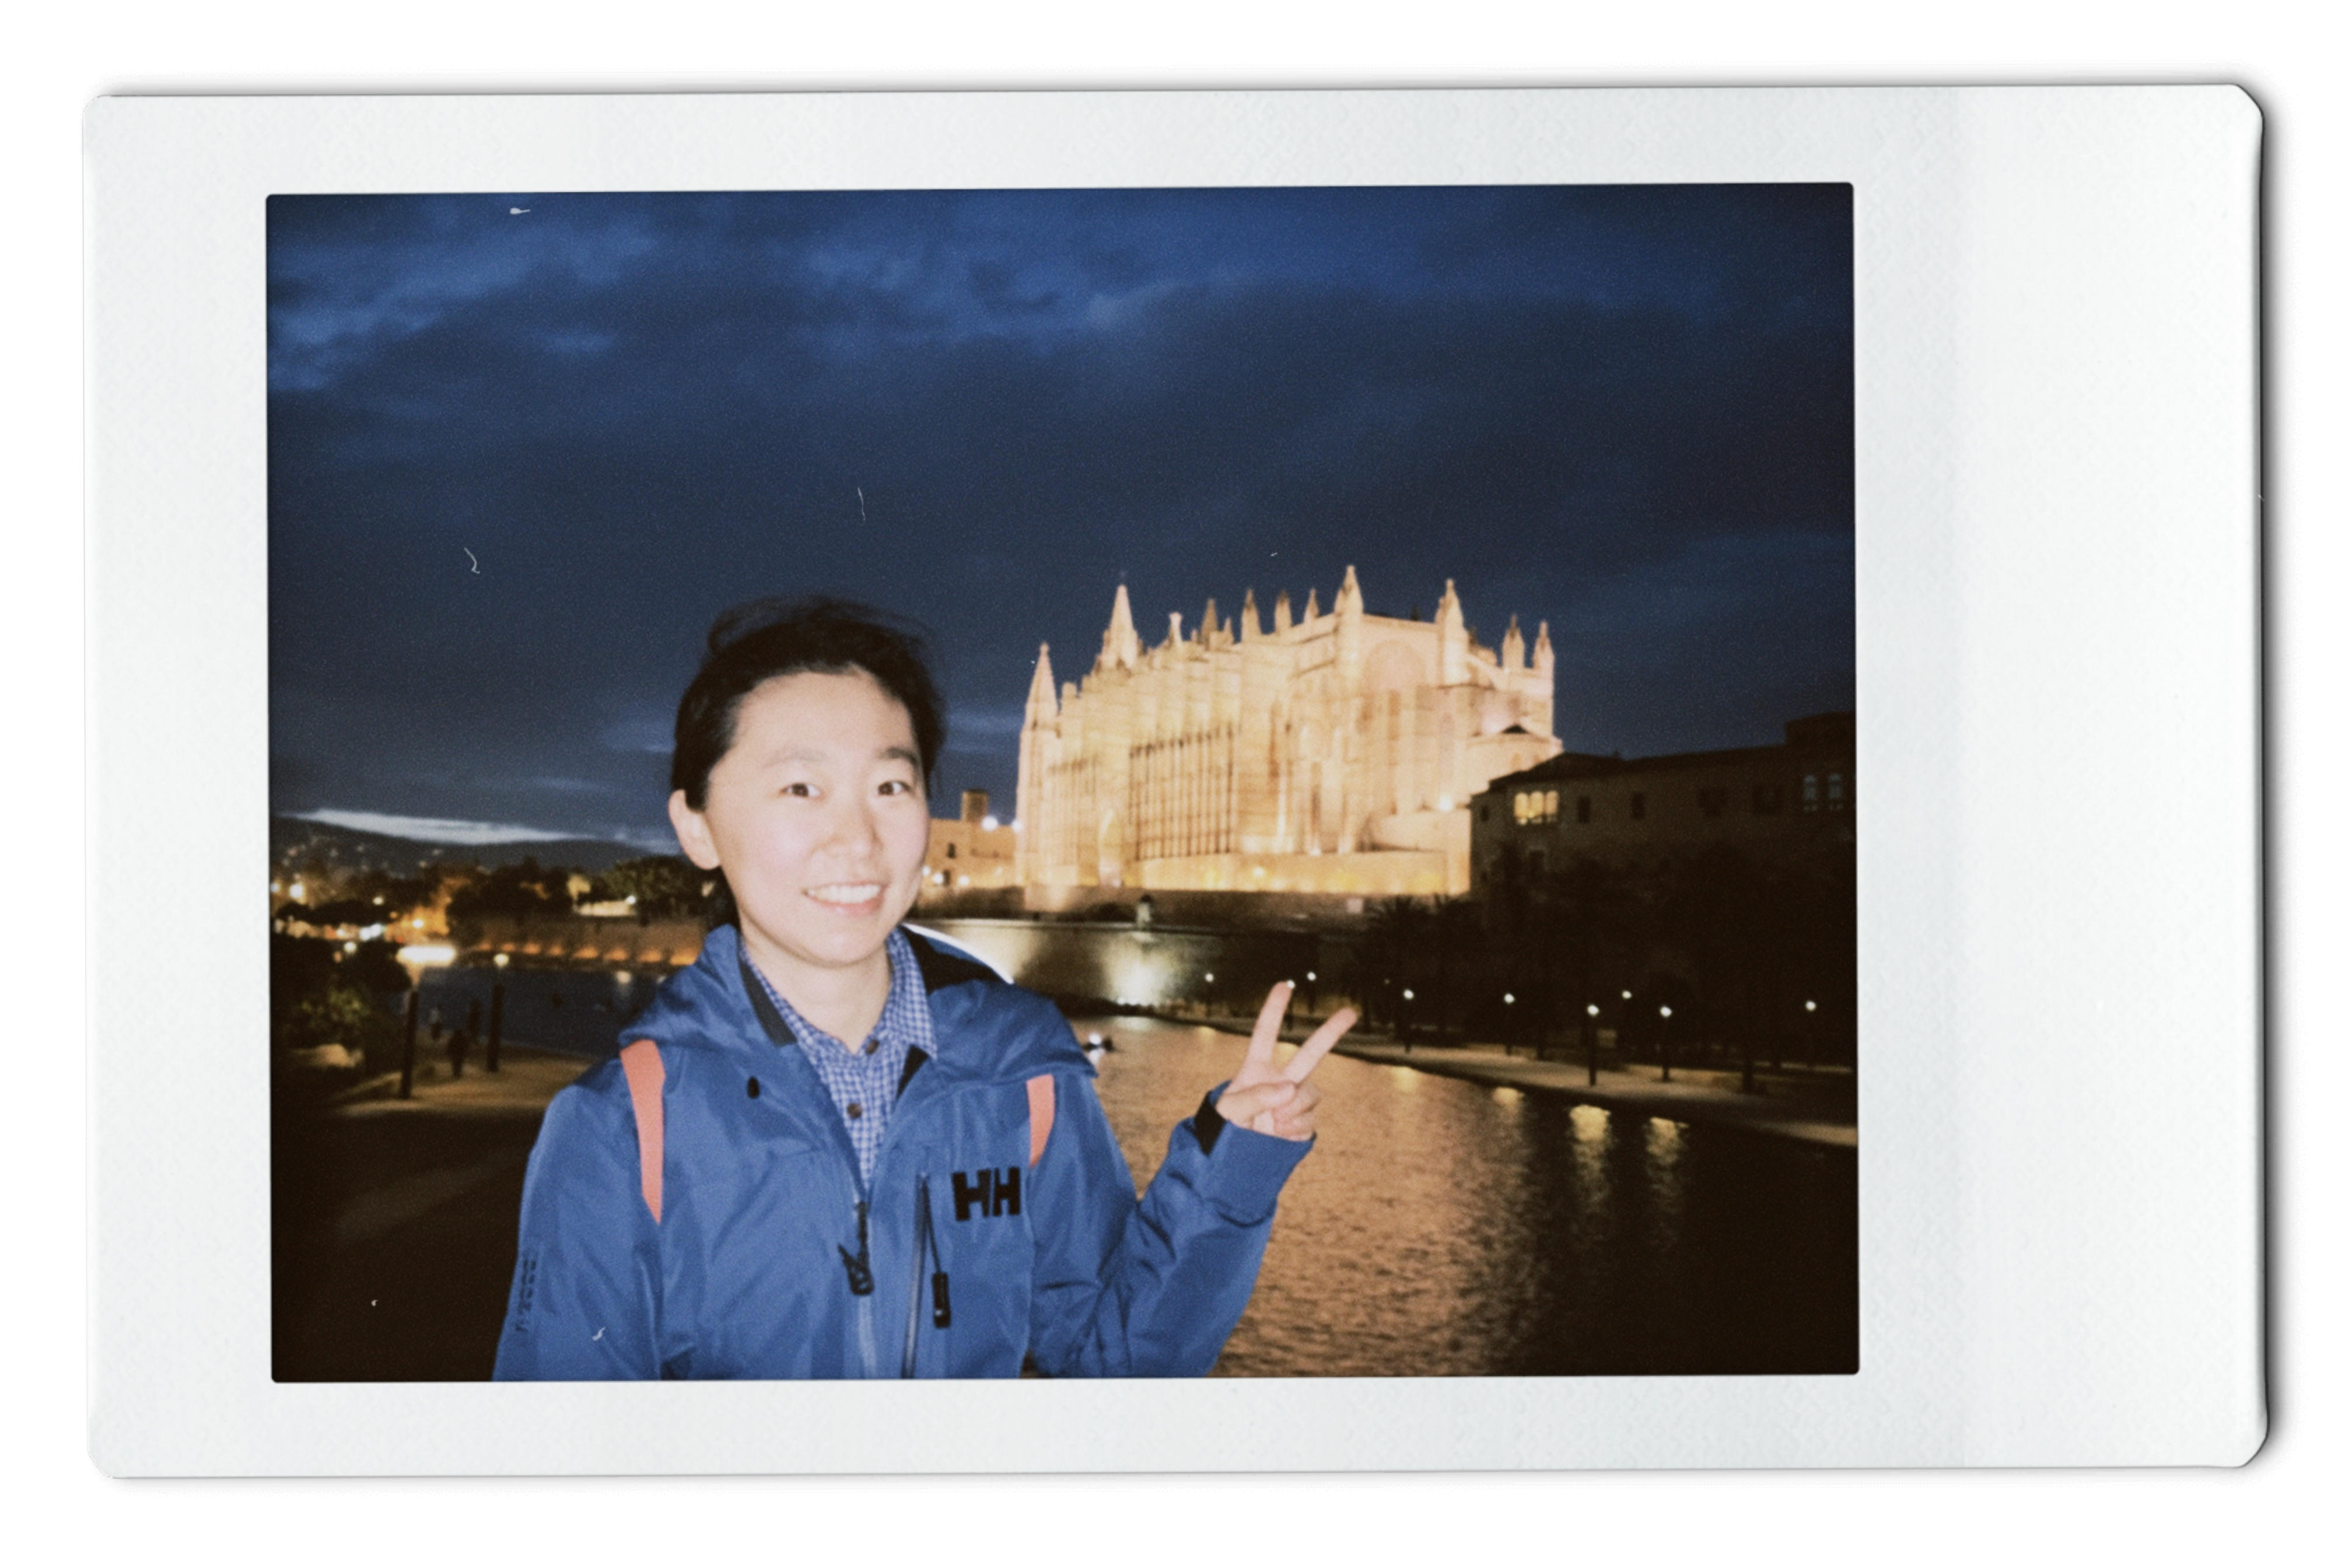
\includegraphics[width=5.21875in,height=\textheight,keepaspectratio]{images/clipboard-3563974152.jpeg}
\end{center}

In this diary after exploring various global case studies in the initial
weeks, I decided to shift my focus closer to my hometown, Beijing, as
the primary study area. Leveraging Earth observation data allows me to
step outside my everyday, ground-level experience and gain fresh,
data-driven insights into a city I thought I knew so well.

\section*{Contents}\label{contents}
\addcontentsline{toc}{section}{Contents}

\markright{Contents}

In this diary, I will cover the summary, applications, and my own
reflections on each week of the module with the following structure:

\textbf{Week 1}: Getting started with remote sensing

\textbf{Week 2}: Landsat xaringan presentation

\textbf{Week 3}: Feature Extraction and Dimension Reduction

\textbf{Week 4}: Policy

\textbf{Week 5}: Meet Earth Google Engine

\textbf{Week 6:} Classification 1

\textbf{Week 7}: Classification 2

\textbf{Week 8}: Temperature

\bookmarksetup{startatroot}

\chapter{Getting started with remote
sensing}\label{getting-started-with-remote-sensing}

\section{Summary}\label{summary}

``This week's content has shifted my perspective on remote sensing
imagery from merely `aesthetic images' to \textbf{quantifiable spectral
data}. Different land covers---such as water, vegetation, and
buildings---possess unique \textbf{spectral response characteristics},
exhibiting significant variations across different bands. Sensors, in
essence, capture the \textbf{radiance or reflectance information} of the
Earth's surface across the electromagnetic spectrum.''

\subsection{Four types of resolution}\label{four-types-of-resolution}

\begin{itemize}
\item
  \textbf{Spatial Resolution}: A smaller pixel size provides finer
  detail, whereas a larger pixel size is more prone to the mixed pixel
  effect.
\item
  \textbf{Spectral Resolution}: Refers to the number and width of
  spectral bands. Narrower and more numerous bands allow for better
  differentiation of subtle spectral signatures between materials.
\item
  \textbf{Temporal Resolution}: The frequency of repeat observations
  over the same area.
\item
  \textbf{Radiometric Resolution}：This resolution defines the sensor's
  sensitivity to changes in light intensity. By quantizing the received
  energy into finer brightness levels, higher resolution results in much
  smoother color or grayscale transitions.
\end{itemize}

\subsection{Feature Identification}\label{feature-identification}

Utilizing QGIS and SNAP, I employed true-color/false-color composites
and histogram stretching to rapidly identify the spatial patterns of
water bodies, vegetation, and built-up areas. This process enabled a
direct comparison of the differences in scale and level of detail
between Sentinel and Landsat imagery. Beyond mere visual observation,
this step involves a quality screening for issues such as cloud cover,
shadows, stripping, and edge NoData values, providing a \textbf{basis}
for defining AOIs and sampling strategies in subsequent stages.

\section{Applications}\label{applications}

\subsection{\texorpdfstring{\textbf{Processing
levels}}{Processing levels}}\label{processing-levels}

The most common classification for mainstream remote sensing products is
based on their processing levels. Specifically, NASA's Level 0--4
definitions serve as the widely adopted reference framework across the
industry
\href{https://www.earthdata.nasa.gov/learn/earth-observation-data-basics/data-processing-levels?utm_source=chatgpt.com}{NASA
Data Processing Levels Processing Levels}.

\begin{longtable}[]{@{}
  >{\raggedright\arraybackslash}p{(\linewidth - 4\tabcolsep) * \real{0.2192}}
  >{\raggedright\arraybackslash}p{(\linewidth - 4\tabcolsep) * \real{0.2192}}
  >{\raggedright\arraybackslash}p{(\linewidth - 4\tabcolsep) * \real{0.5616}}@{}}
\caption{Remote Sensing Data Processing Levels}\tabularnewline
\toprule\noalign{}
\begin{minipage}[b]{\linewidth}\raggedright
Level
\end{minipage} & \begin{minipage}[b]{\linewidth}\raggedright
Name
\end{minipage} & \begin{minipage}[b]{\linewidth}\raggedright
Key definitions
\end{minipage} \\
\midrule\noalign{}
\endfirsthead
\toprule\noalign{}
\begin{minipage}[b]{\linewidth}\raggedright
Level
\end{minipage} & \begin{minipage}[b]{\linewidth}\raggedright
Name
\end{minipage} & \begin{minipage}[b]{\linewidth}\raggedright
Key definitions
\end{minipage} \\
\midrule\noalign{}
\endhead
\bottomrule\noalign{}
\endlastfoot
L0 & Raw Data & Raw sensor streams, typically as original telemetry
packets. \\
L1 & Geometric Correction & Data is converted to physical units with
Earth location information attached. \\
L2 & Surface Physical Variables & Derived geophysical variables. The
most critical step is Atmospheric Correction \\
L3 & Spatio-temporal Composites & Mapped and gridded variables. Data is
resampled onto a global or regional grid, often involving spatial
mosaicking and temporal compositing. \\
L4 & Higher-level Analysis Products & Integrated output from models. \\
\end{longtable}

\subsection{Key Sensors}\label{key-sensors}

\begin{itemize}
\item
  \textbf{Sentinel-1 (SAR)}, with its cloud-penetrating and
  day-and-night imaging capabilities, is the preferred choice for event
  monitoring in cloudy or disaster-stricken scenarios.
\item
  \textbf{Sentinel-2} is better suited for fine-grained surface
  interpretation, such as urban textures, detailed vegetation and water
  distribution, or short-term changes.
\item
  \textbf{Landsat}'s long-term data record and stable calibration make
  it ideal for \textbf{lo}ng-term trend analysis, including decadal
  land-use changes and urban expansion.
\item
  \textbf{MODIS and VIIRS} excel due to their high temporal resolution,
  capturing seasonal dynamics and regional indicators.
\end{itemize}

\section{Reflection}\label{reflection}

I used to rely more on QGIS/SNAP because it is highly intuitive: by
switching a band combination or applying a simple stretch, differences
between land-cover types become visible immediately. It is also easier
to spot issues such as cloud and shadow contamination. However, this
week I realised that as the data scale grows, the strengths of SNAP can
turn into limitations: the same steps must be repeated manually, the
workflow is harder to standardise, and it becomes more difficult to
ensure consistent processing choices across runs. By contrast,
code-based approaches feel more abstract at first, because they require
translating what I do in the software into variables, parameters, and
functions. Yet once the workflow is scripted, it can be run in batch,
reused across datasets, and every processing decision is recorded. Going
forward, an ideal strategy for me is to use the SNAP for rapid
exploration and quality control, while relying on code for reproducible,
scalable batch processing and quantitative analysis---reducing
repetitive work and improving the reliability of my research.

\bookmarksetup{startatroot}

\chapter{Landsat xaringan
presentation}\label{landsat-xaringan-presentation}

\bookmarksetup{startatroot}

\chapter{Feature Extraction and Dimension
Reduction}\label{feature-extraction-and-dimension-reduction}

\section{Summary}\label{summary-1}

This learning task uses Landsat satellite imagery of Cape Town as its
basis. Using the R programming language, we extracted the Normalized
Difference Vegetation Index (NDVI) based on spectral features and
calculated the Gray-Level Co-occurrence Matrix (GLCM) texture based on
spatial features. Finally, we performed dimensional reduction and
extracted key features from the multi-source fused data using Principal
Component Analysis (PCA). This week's learning theme focuses on
``Advanced Feature Extraction and Data Dimension Reduction.'' The
primary objective of performing this series of preprocessing operations
is to prepare the most concise and highest-quality feature variables for
subsequent land cover classification (or machine learning models).

\subsection{NDVI: Vegetation Feature
Extraction}\label{ndvi-vegetation-feature-extraction}

Based on the principle that different surface materials reflect light
differently (healthy vegetation contains chlorophyll, which strongly
absorbs red light, while the cellular structure of plants strongly
reflects near-infrared light), the calculation is performed using the
following formula: \[NDVI = \frac{B5 - B4}{B5 + B4}\]

\begin{figure}[H]

{\centering \pandocbounded{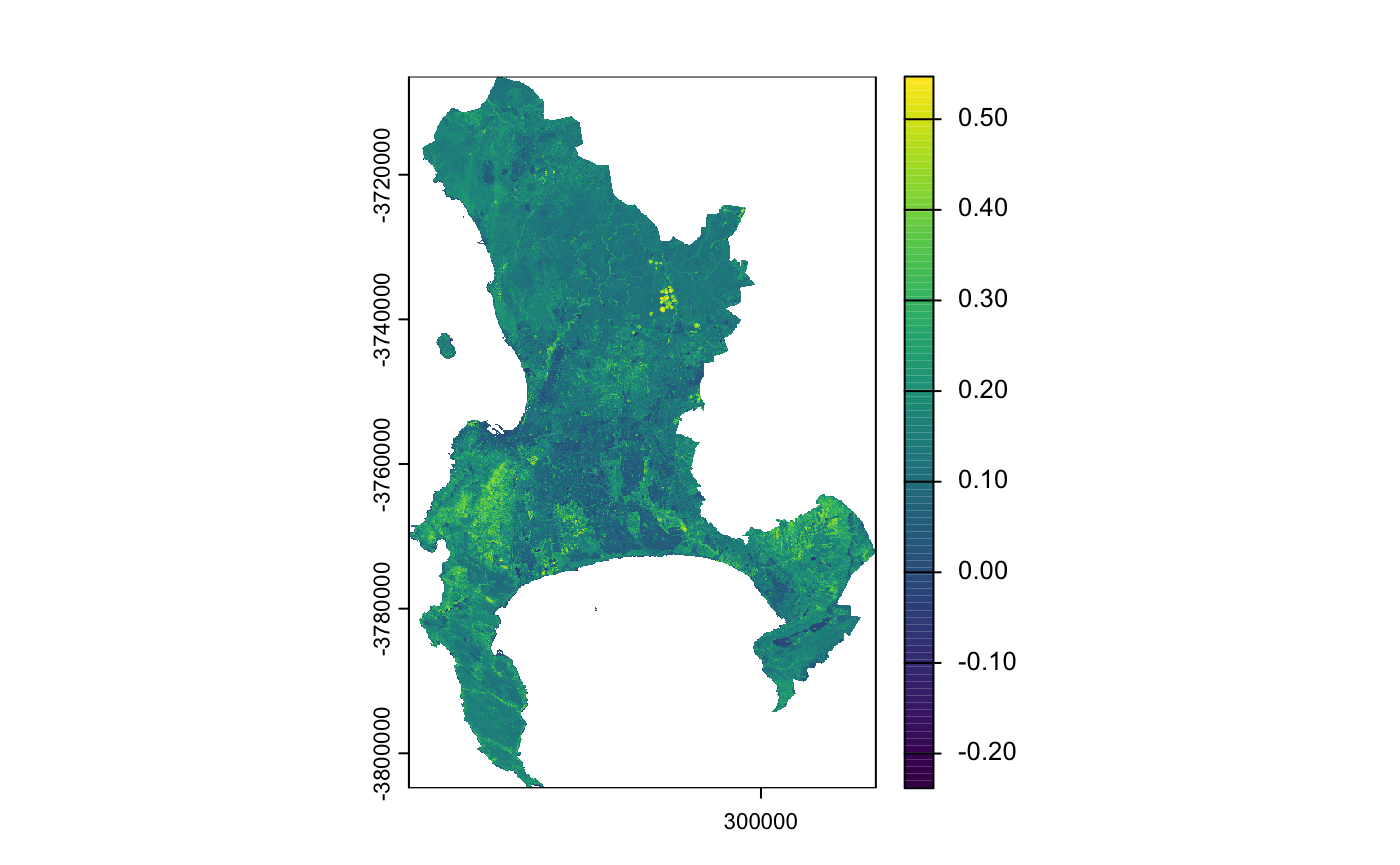
\includegraphics[keepaspectratio]{week3/images/clipboard-3431523994.png}}

}

\caption{Cape Town NDVI}

\end{figure}%

In the analysis of the Cape Town region, after calculating the NDVI for
the entire area, we set a threshold of 0.2. By masking areas with values
below this threshold, we successfully removed large areas of
non-vegetation backgrounds, such as the ocean, dense urban structures,
and bare soil. This process yielded a clean, valid vegetation cover map.

\begin{figure}[H]

{\centering \pandocbounded{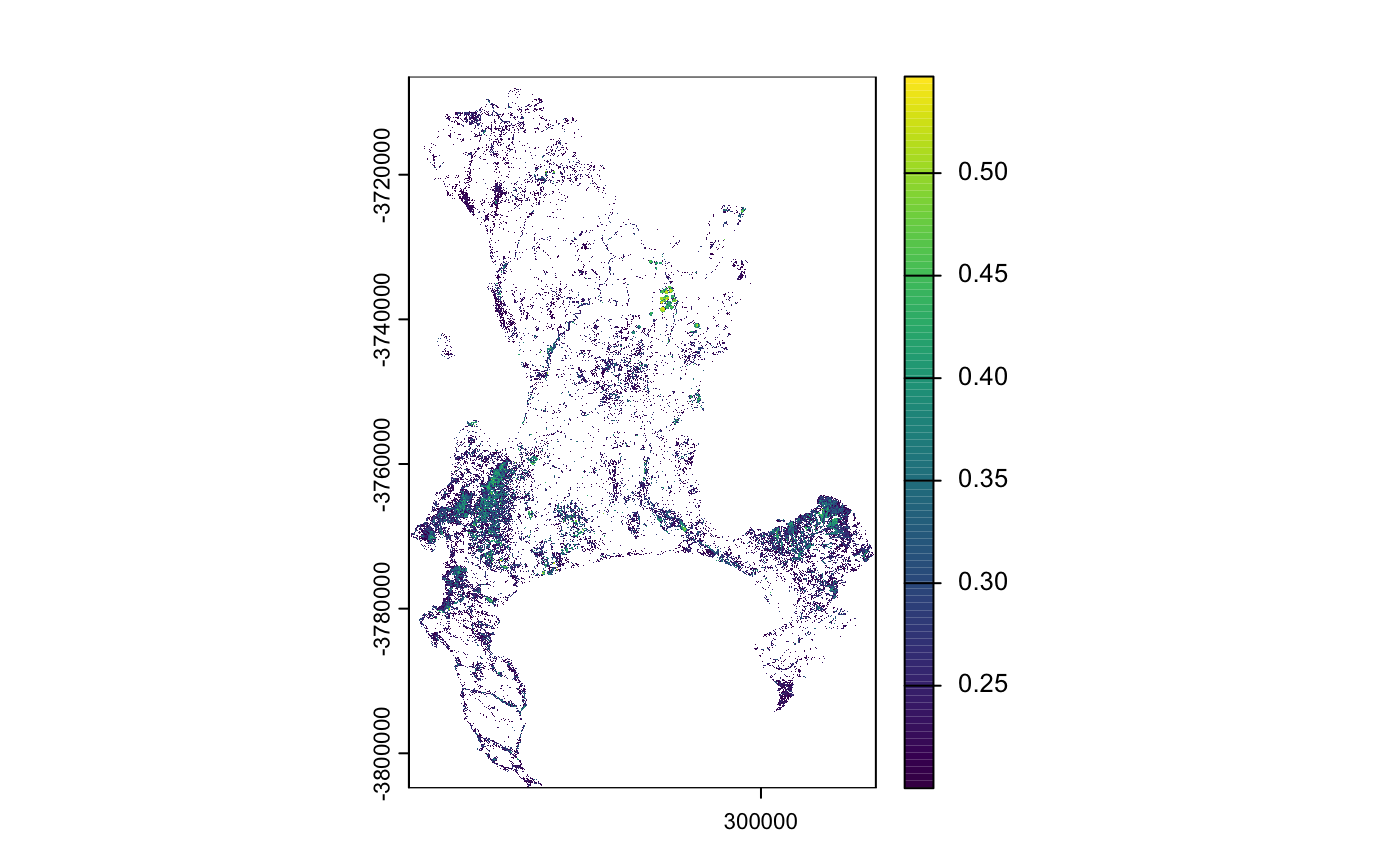
\includegraphics[keepaspectratio]{week3/images/clipboard-3663781118.png}}

}

\caption{Cape Town NDVI}

\end{figure}%

\subsection{GLCM: Spatial Texture Feature
Extraction}\label{glcm-spatial-texture-feature-extraction}

Satellite spectral bands mainly reflect surface color, but not spatial
structure. Gray-Level Co-occurrence Matrix (GLCM) quantifies texture by
analyzing grey-level variations between neighboring pixels, capturing
surface smoothness or roughness.

The formula for converting DN to refractive index is：
\(\rho = (DN \times 0.0000275) - 0.2\)）

In this study, using Cape Town as an example, we calculated a 7×7 window
homogeneity metric from the red band. The large areas of light gray and
pure white in the image represent ``high homogeneity,'' indicating that
the surface in these areas is smooth, such as open water bodies,
vegetation, or flat bare ground. The dark gray, densely spotted areas
represent ``low homogeneity,'' indicating that the texture of the
adjacent surface is fragmented, corresponding to urban built-up areas,
dense residential zones.

\begin{figure}[H]

{\centering \pandocbounded{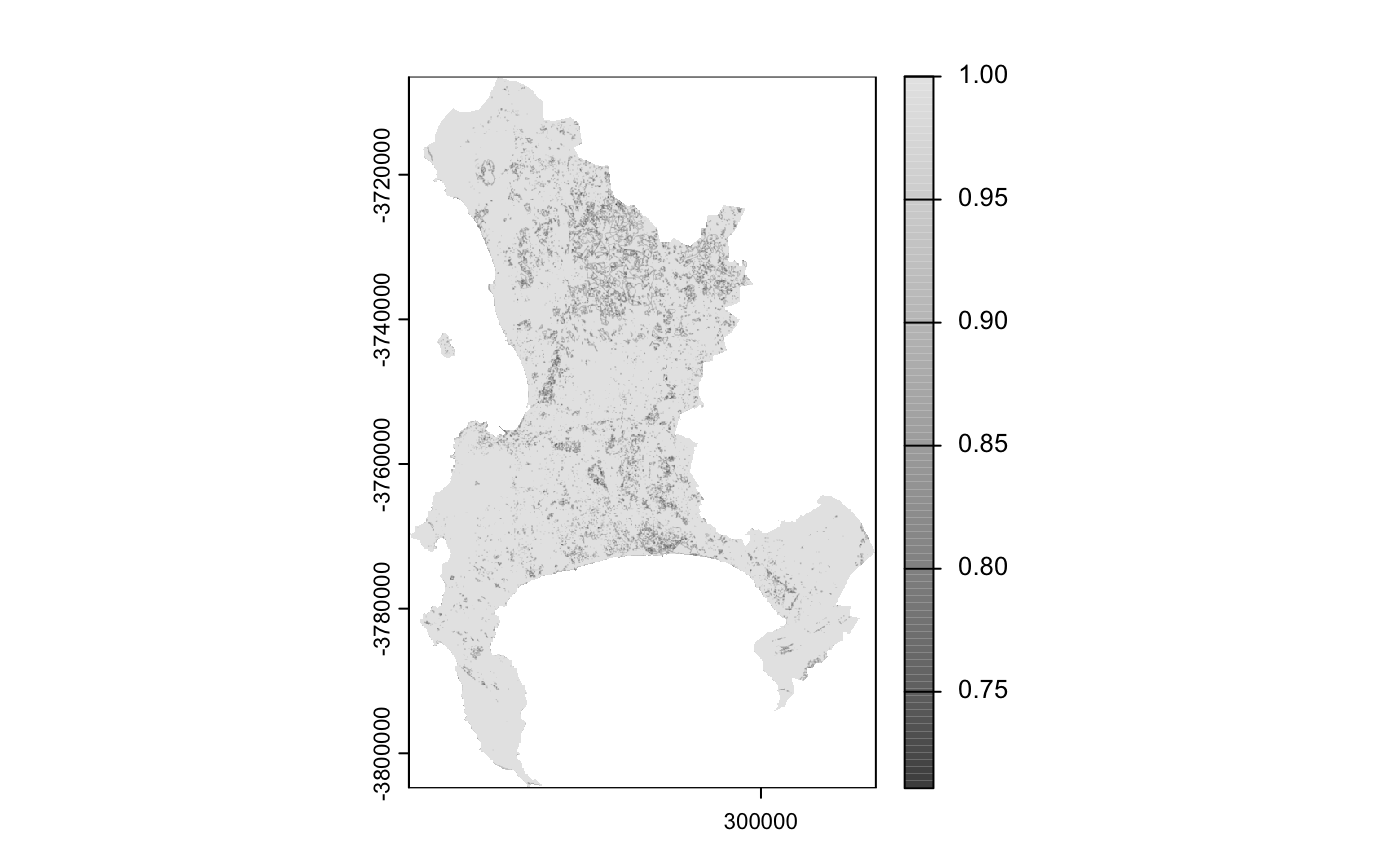
\includegraphics[keepaspectratio]{week3/images/clipboard-4038221735.png}}

}

\caption{Texture for Cape Town}

\end{figure}%

\subsection{PCA: Multi-source Data Fusion and Dimension
Reduction}\label{pca-multi-source-data-fusion-and-dimension-reduction}

There is typically a strong correlation between the various bands in
multispectral imagery, leading to information redundancy and introducing
a certain amount of noise. PCA uses an orthogonal transformation to
convert these correlated layers into a set of mutually independent new
variables, which are ranked by information content.

We applied PCA to eight spectral bands and one texture band from Cape
Town. Most of the useful information is captured in the first few
components, while noise and less important variation are pushed into
later components. This helps reduce redundancy and provides clearer
inputs for land cover classification.

\begin{figure}[H]

{\centering \pandocbounded{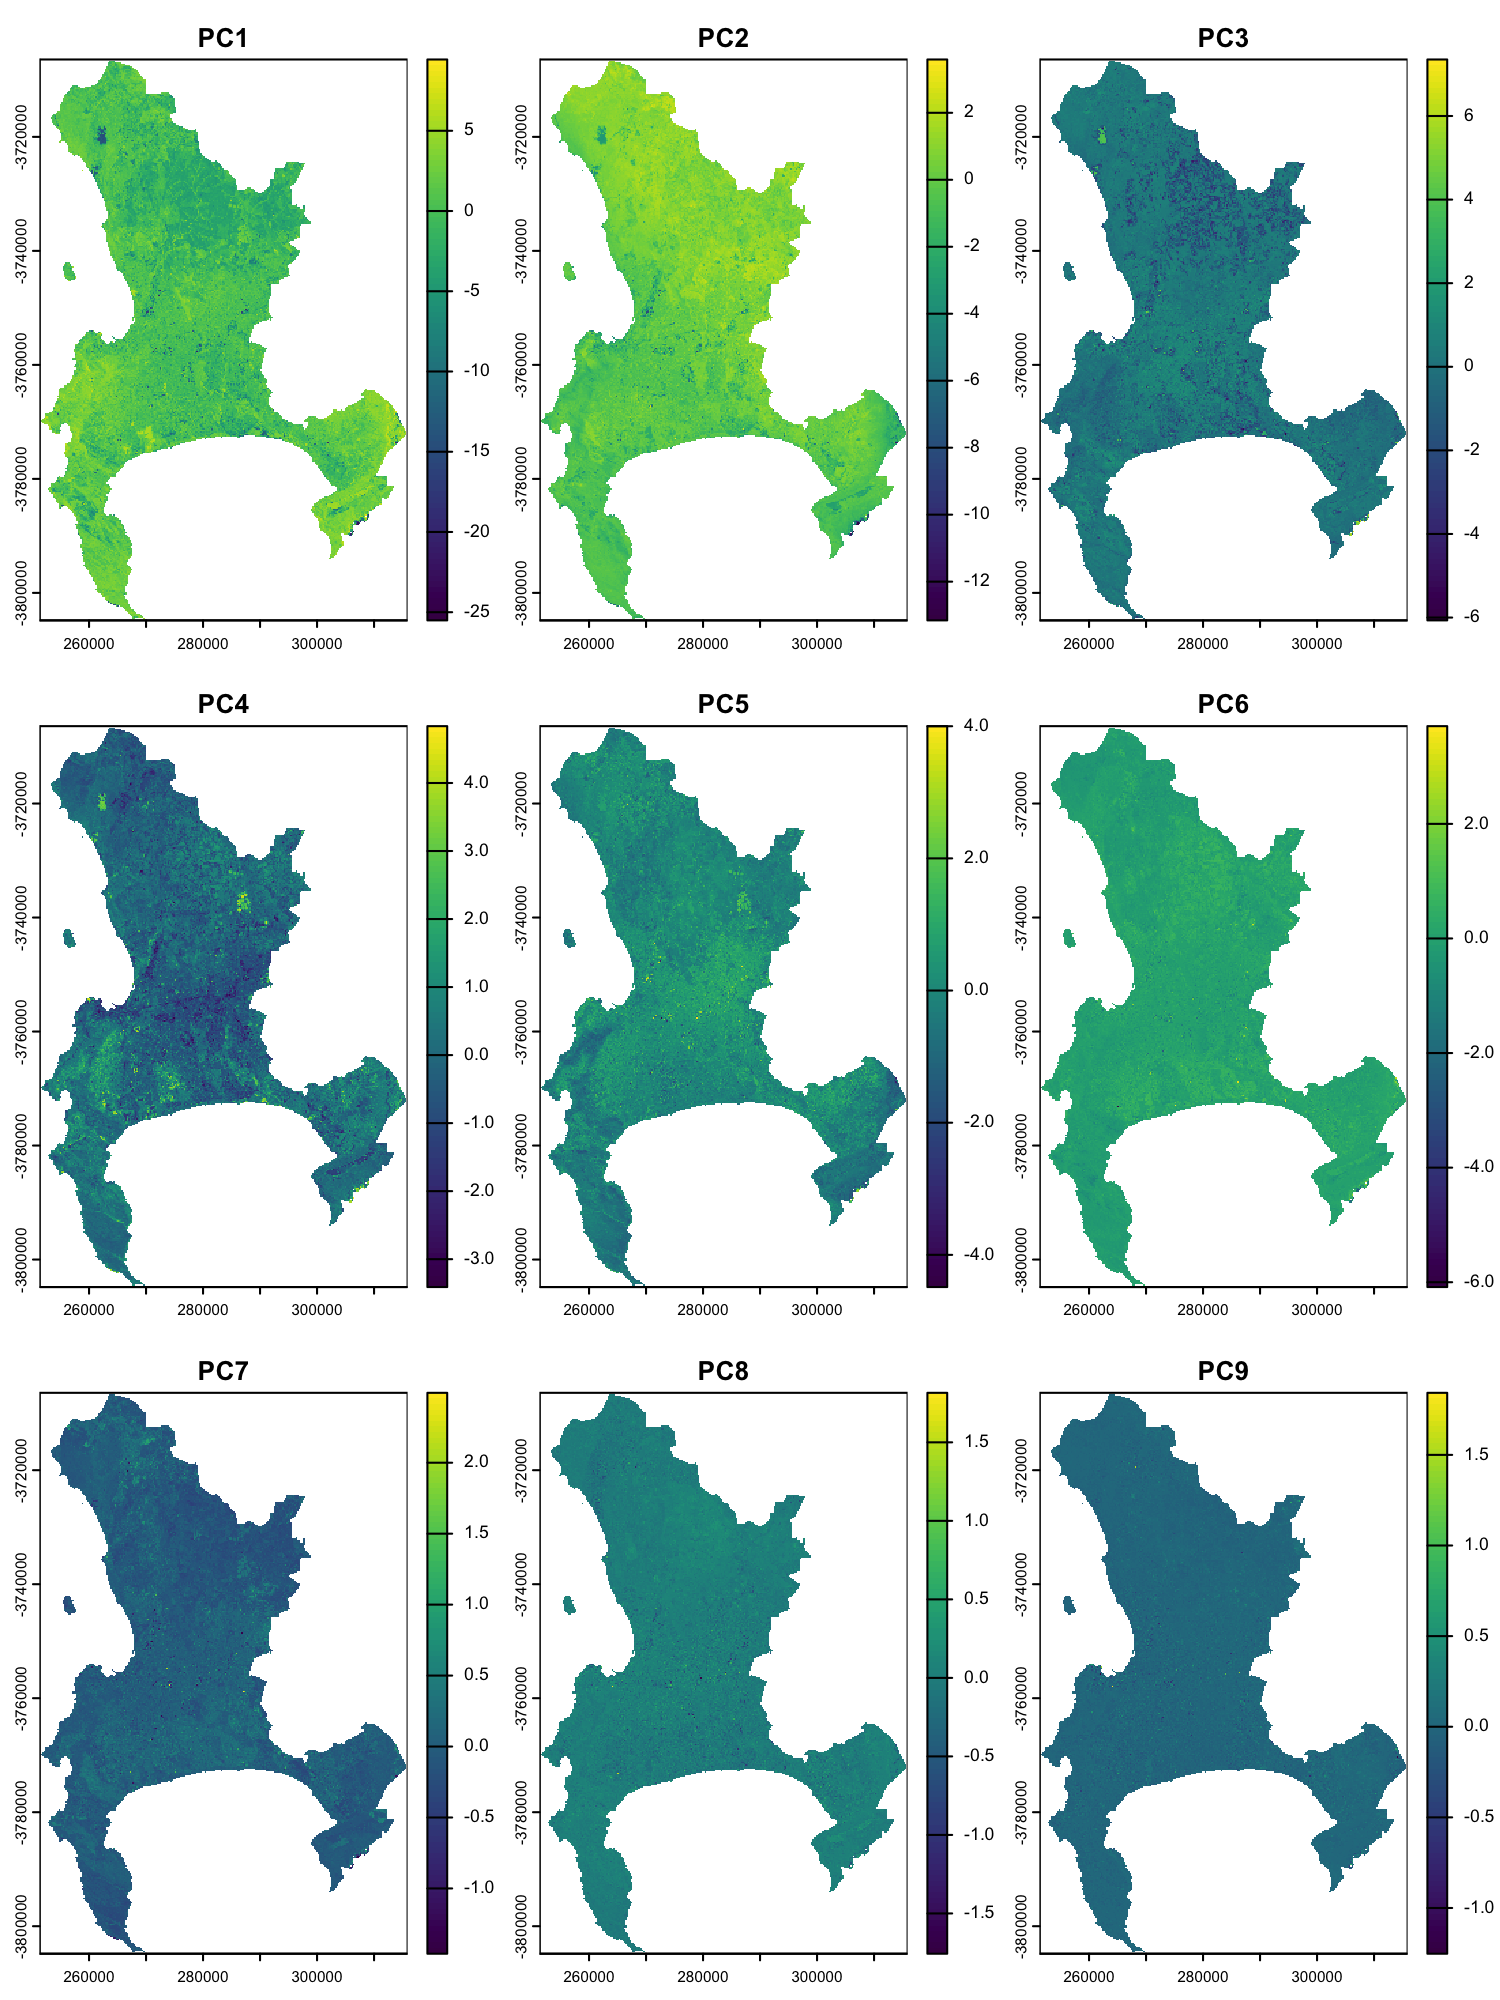
\includegraphics[keepaspectratio]{week3/images/PCA_perfect.png}}

}

\caption{PCA for Cape Town}

\end{figure}%

\section{Application}\label{application}

Principal Component Analysis (PCA), as a preprocessing step for
dimensionality reduction, has been widely applied in remote sensing
workflows. For example, (Zabalza et al. 2014) incorporated PCA into a
broader feature extraction framework for hyperspectral and Synthetic
Aperture Radar (SAR) data. PCA was primarily used to reduce data
dimensionality and computational load.

Several recent studies have combined PCA with convolutional neural
networks (CNNs). PCA is used to reduce spectral redundancy, while CNNs
extract spatial features and perform classification. This approach
significantly improves classification accuracy compared to traditional
methods(Roy et al. 2020). Essentially, the capabilities of PCA itself
have not been enhanced; rather, the introduction of CNNs compensates for
PCA's limitations in representing spatial information.

\begin{figure}[H]

{\centering \pandocbounded{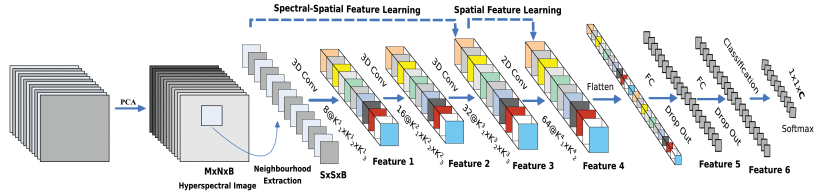
\includegraphics[keepaspectratio]{week3/images/clipboard-1486884527.png}}

}

\caption{Proposed HybridSpectralNet (HybridSN) model that integrates 3-D
and 2-D convolutions for HSI classification.(Roy et al. 2020)}

\end{figure}%

In addition, some studies have developed more complex processing
workflows by combining PCA with multi-stage feature extraction
techniques, thereby capturing both global and local features of the data
simultaneously. This suggests that in modern remote sensing analysis,
PCA is more commonly used as a dimension-reduction tool rather than as a
standalone feature extraction method.

\begin{itemize}
\tightlist
\item
  \textbf{PCA + Spatial-Spectral Fusion:} Fusing the global features
  extracted by PCA with the local features extracted by SSA
  significantly improves the accuracy of land cover classification.(Wang
  et al. 2021)
\end{itemize}

\begin{figure}[H]

{\centering \pandocbounded{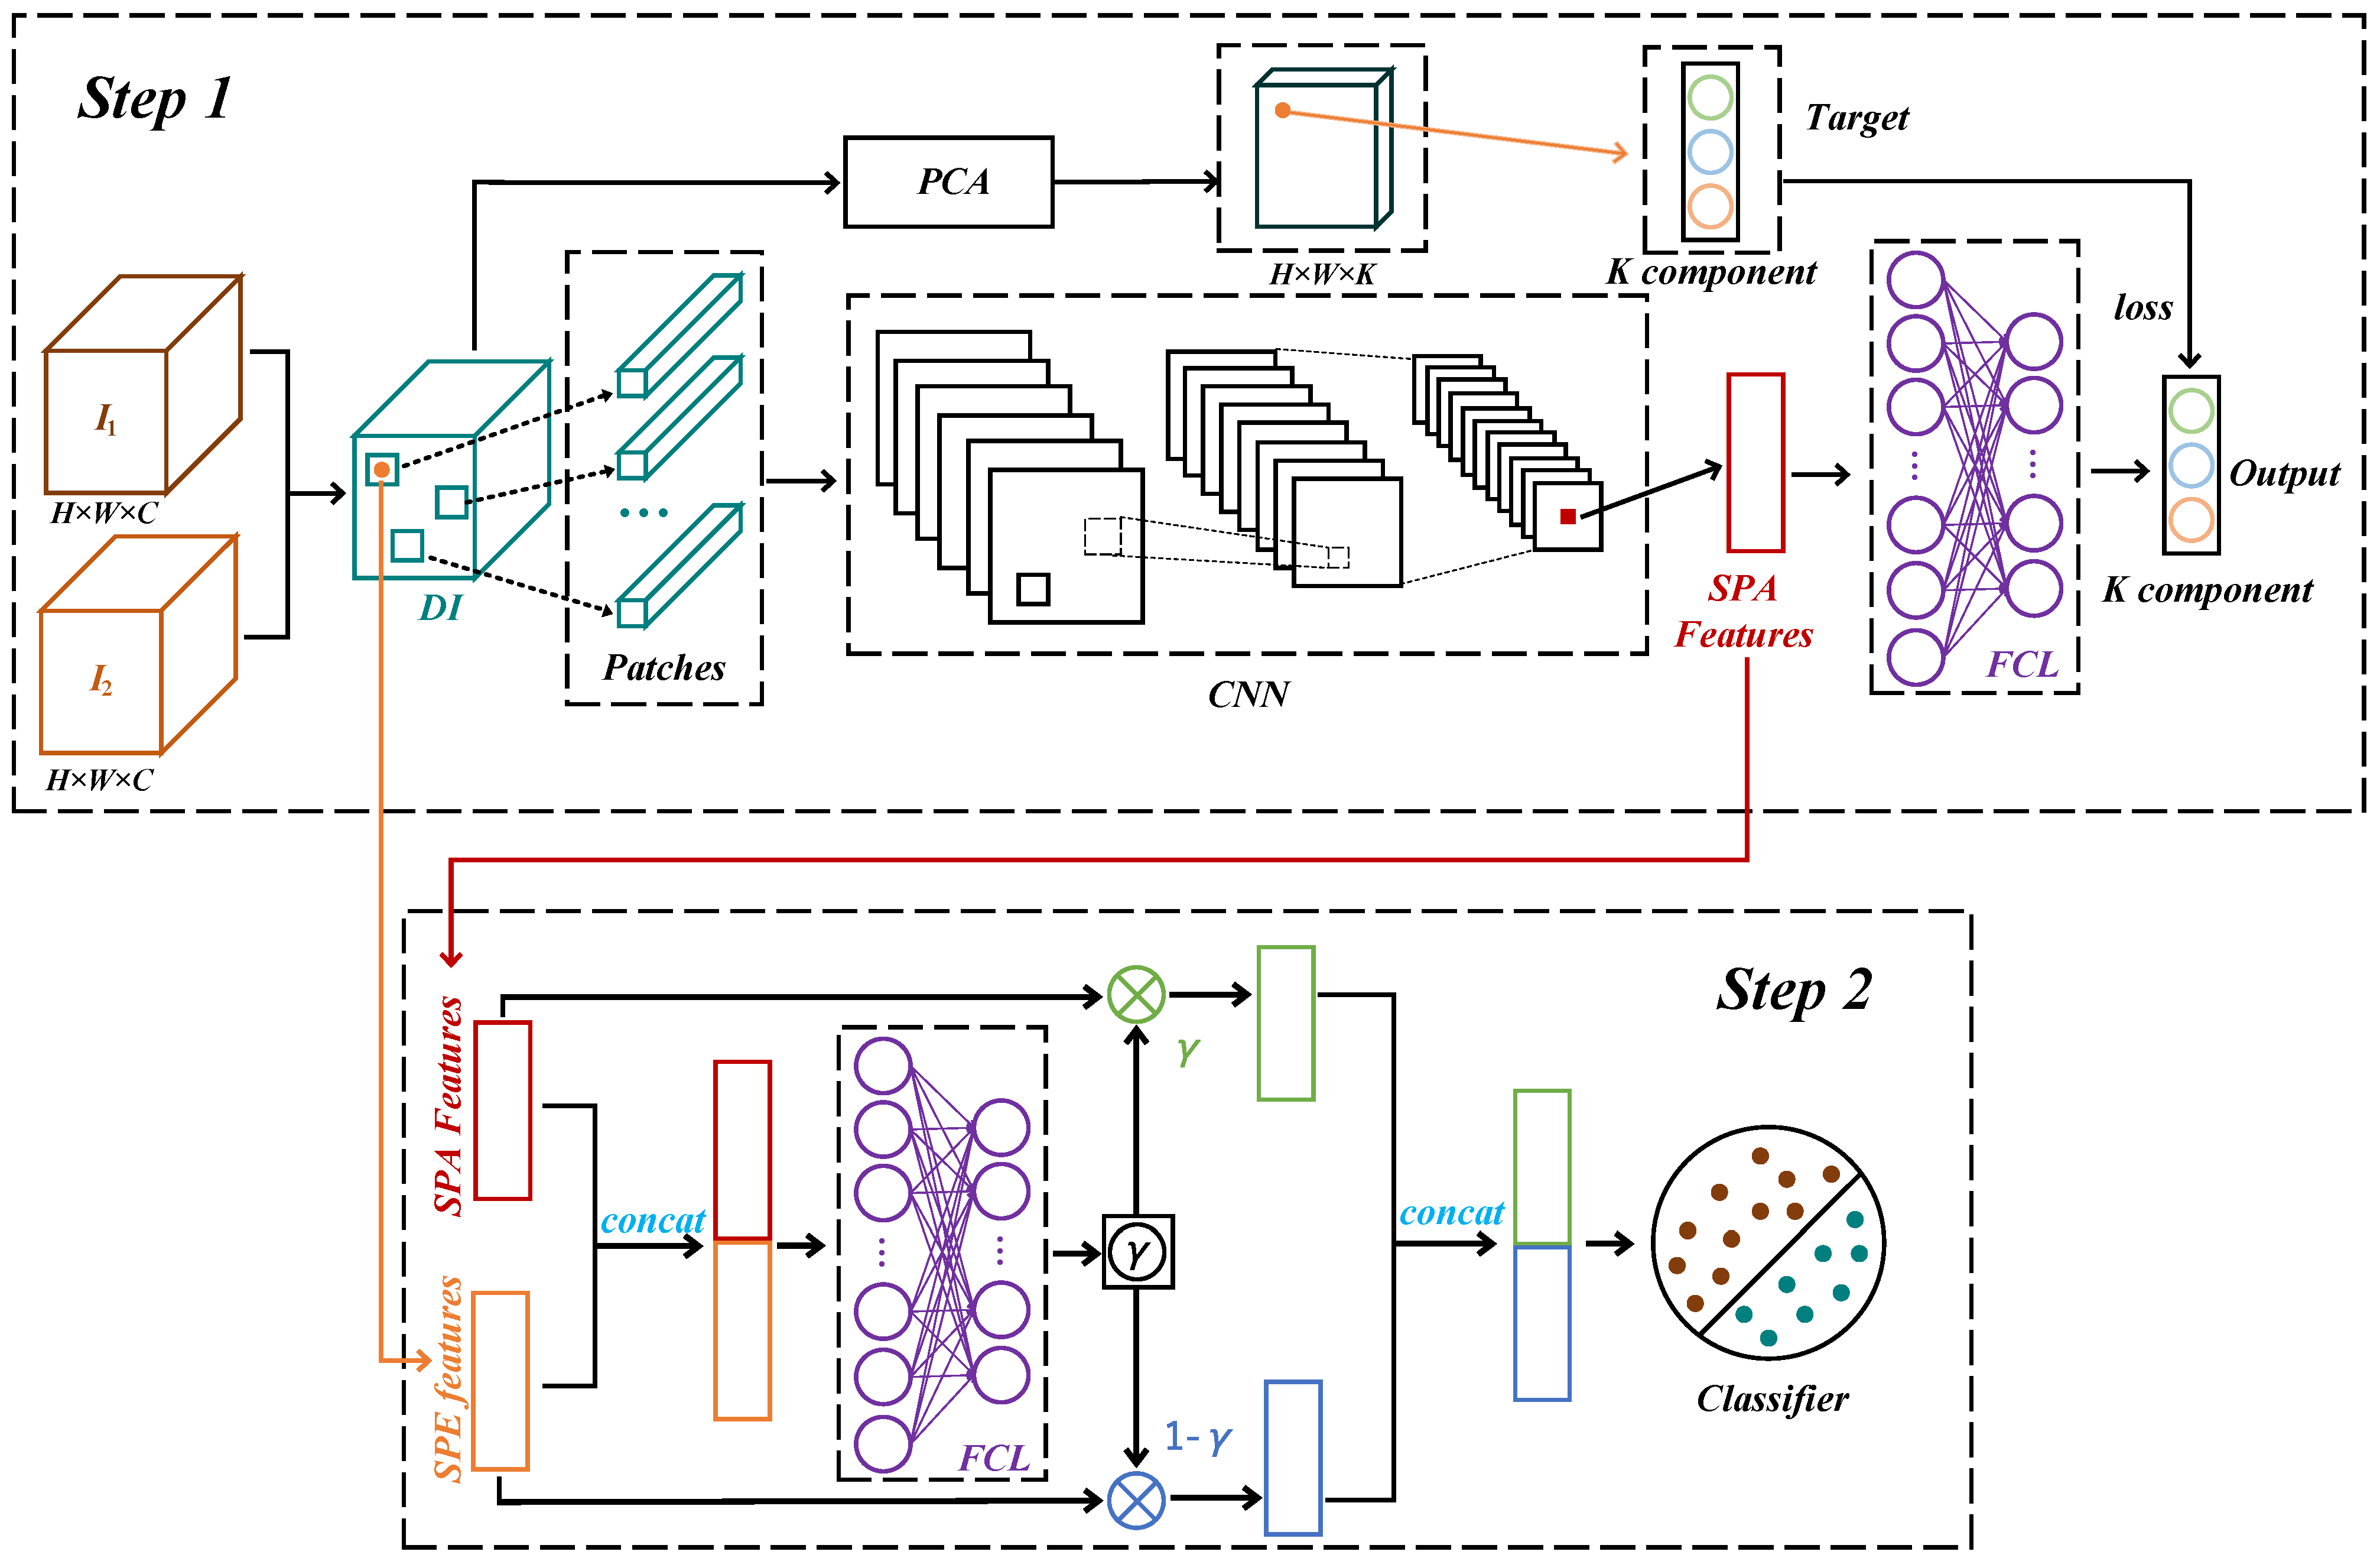
\includegraphics[keepaspectratio]{week3/images/clipboard-1812895644.png}}

}

\caption{Framework of the proposed ASSCDN.(Wang et al. 2021)}

\end{figure}%

\begin{itemize}
\tightlist
\item
  \textbf{PCA + Hybrid Manifold Learning:} Within PCA, apply LPP
  (Locally Linear Embedding) or t-SNE to preserve the local geometric
  proximity of the data(Cao et al. 2024).
\end{itemize}

\section{Reflection}\label{reflection-1}

Through practical experience, I have found that PCA has some obvious
drawbacks. For example, PCA combines the original features linearly into
new principal components, which means the results lack intuitive
physical or practical meaning. While the plot shows which directions
exhibit the greatest variation, it is impossible to clearly determine
which light waves are responsible for these changes. Furthermore, since
PCA prioritizes retaining information with large variations, useful
information may be lost in some practical tasks where features with
small variations are often equally important for classification or
recognition. Overall, while PCA effectively compresses information, its
poor interpretability and insensitivity to nonlinearities and
small-amplitude changes are limitations that must be weighed when using
the method.

\bookmarksetup{startatroot}

\chapter{Policy}\label{policy}

\section{Introduction}\label{introduction-1}

Ahmedabad is one of India's typical high-temperature cities and has
experienced frequent extreme heat waves over the past few decades. As
urbanization progresses, the increase in impervious surfaces and the
reduction in green spaces have further exacerbated the urban heat island
effect. After analyzing data from 2002 to 2018, (A. Sharma et al. 2024)
found a significant association between extreme heat events and
all-cause mortality. Extreme heat is no longer merely a climatic
phenomenon; it poses a substantial threat to public health.

\begin{figure}[H]

{\centering 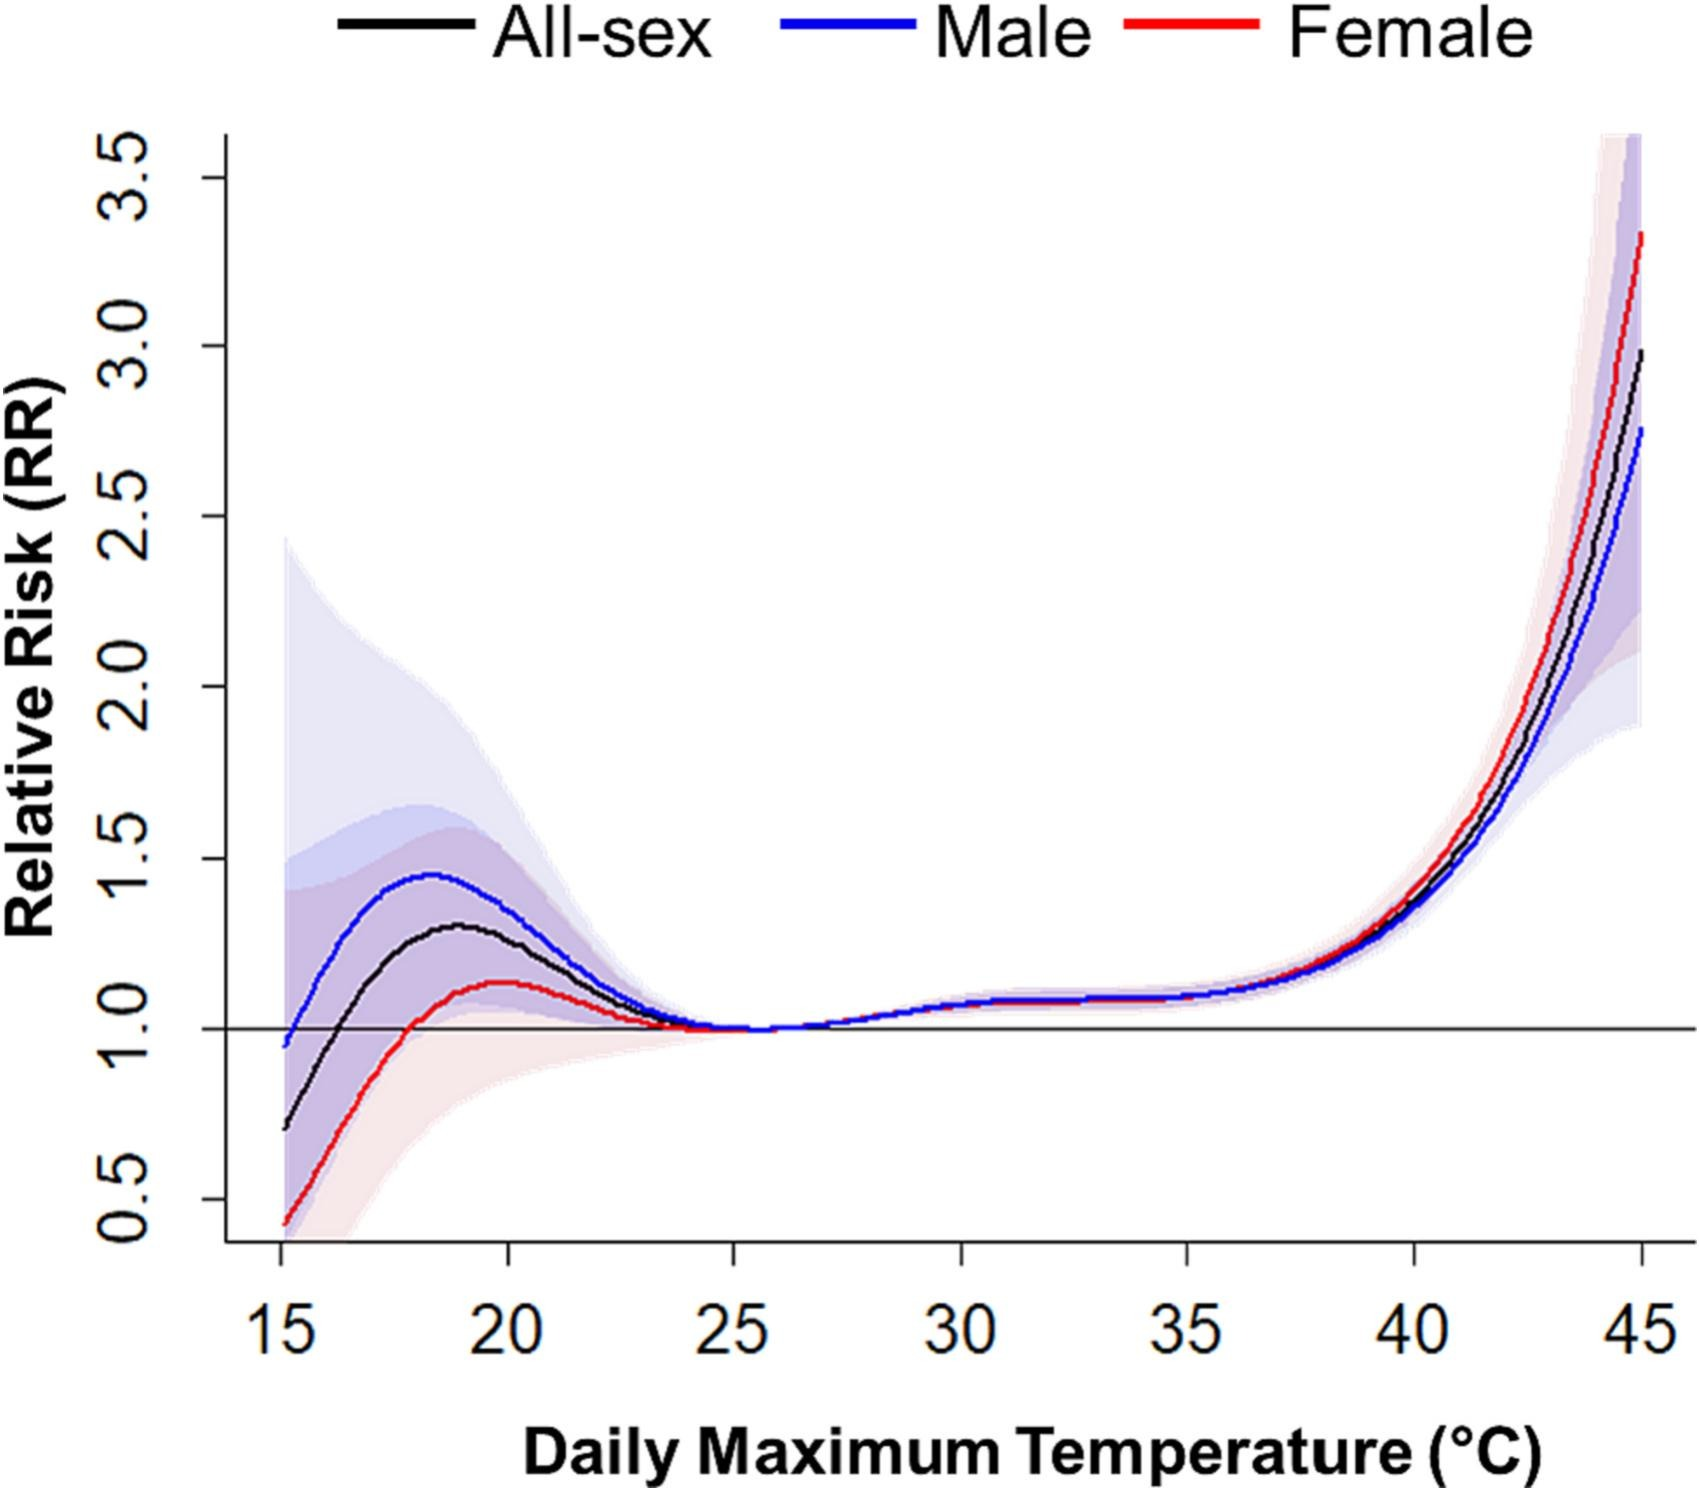
\includegraphics[width=4.66667in,height=\textheight,keepaspectratio]{images/clipboard-2170059669.png}

}

\caption{Association between Maximum Temperature and Mortality Risk.
Resource: (A. Sharma et al. 2024).}

\end{figure}%

\section{Ahmedabad 2016 Heat Action
Plan}\label{ahmedabad-2016-heat-action-plan}

Against this backdrop, Ahmedabad began to gradually explore systematic
measures to address heatwaves, the most notable of which is the
Ahmedabad Heat Action Plan. This policy is considered the first
city-level heat-related health response plan in South Asia. It primarily
aims to reduce the risks through early warning systems, public awareness
campaigns, and interagency collaboration.

\begin{figure}[H]

{\centering 
\includegraphics[width=3.55208in,height=\textheight,keepaspectratio]{images/clipboard-1704754376.png}

}

\caption{Ahmedabad Heat Action Plan 2019}

\end{figure}%

As the policy was implemented, attention gradually turned to its
effectiveness. Research findings indicate that following the policy's
implementation, the risk of heat-related deaths has decreased (Hess et
al. 2018).This result demonstrates that policy interventions can, to
some extent, mitigate the impacts of extreme weather. This has led me to
further consider whether disparities in heat risk persist across
different areas within the city, and whether existing policies are
capable of adequately identifying these disparities.

Current analytical methods remain primarily based on meteorological
warnings and city-wide responses, with relatively limited attention paid
to spatial variations within cities. Differences in vegetation cover,
building density, and socioeconomic conditions across different areas
all influence their sensitivity to high temperatures. Therefore, how to
more precisely identify the distribution of heat risk within cities and
provide support for more targeted interventions has become a topic
worthy of further exploration.

\section{Data}\label{data}

Given the limitations of existing Heat Action Plans in terms of spatial
resolution. The incorporation of remote sensing data can help provide a
better understanding of variations in heat exposure within cities. By
analyzing multi-source remote sensing data, it is possible to identify
which communities are more vulnerable to high temperatures. Furthermore,
by combining this information with data on vegetation cover and water
body distribution, we can pinpoint areas lacking natural factors that
help mitigate heat stress.

The raw data for LST primarily comes from thermal infrared imagery
(TIRS) captured by the Landsat-8 satellite. Surface emissivity is
derived from the thermal infrared band, and surface temperature for each
pixel is estimated through atmospheric correction and radiometric
calibration. Some researchers have further utilized multispectral and
high-resolution imagery to downscale LST to a 10-meter resolution,
capturing spatial variations in the urban thermal environment(S. Sharma
et al. 2023)

\begin{figure}[H]

{\centering 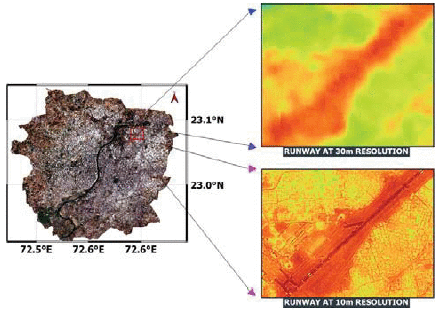
\includegraphics[width=4.94792in,height=\textheight,keepaspectratio]{images/clipboard-1331033014.png}

}

\caption{Visual comparison between 30m and 10m pixel size of ahmedabad
airport runway (tarmac). Resource: (S. Sharma et al. 2023)}

\end{figure}%

Raw NDVI data is derived from the visible and near-infrared bands of
Landsat-8 or Sentinel-2. This index can be used to identify areas within
cities with abundant or scarce green space, and when combined with LST
data, it can be used to analyze the role of green space in mitigating
high temperatures. Previous studies have also shown that vegetation and
water bodies exhibit a negative correlation with surface temperature in
the urban heat environment of Ahmedabad. Areas with abundant vegetation
typically have lower temperatures(Mohammad, Goswami, and Bonafoni 2019).

\begin{figure}[H]

{\centering \pandocbounded{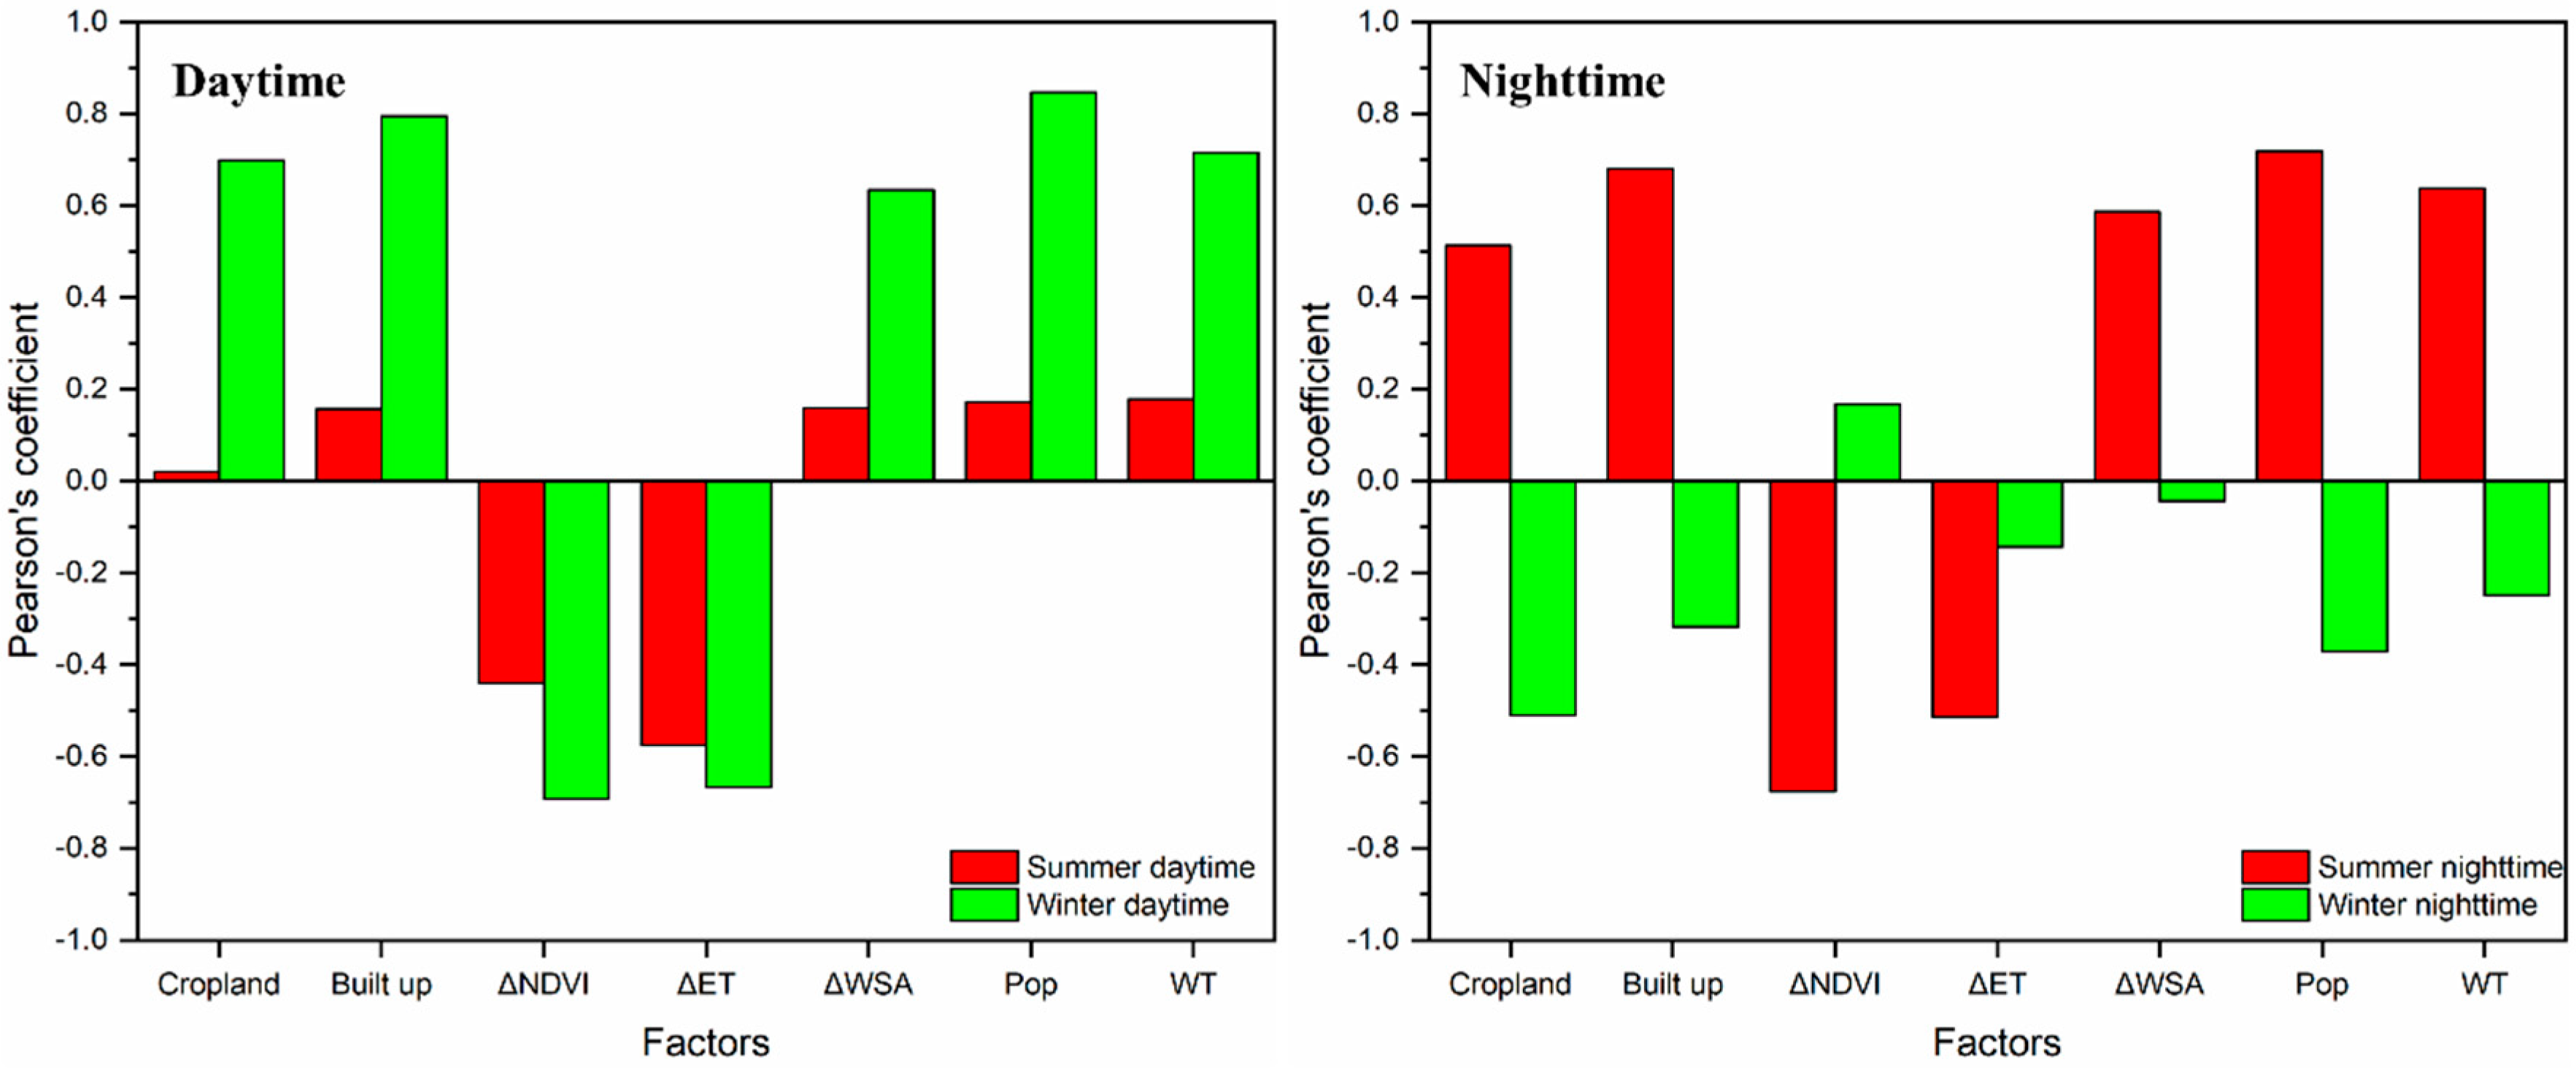
\includegraphics[keepaspectratio]{images/clipboard-2960236245.png}}

}

\caption{Pearson's correlation between SUHII (2003--2018) and different
potential drivers during daytime and nighttime, in the summer and winter
season. (Mohammad, Goswami, and Bonafoni 2019)}

\end{figure}%

\section{Application}\label{application-1}

As we mentioned earlier, we can now obtain Land Surface Temperature
(LST) data with 10-meter resolution and detailed vegetation cover (NDVI)
data. The most direct application of this is to transform these data
into a high-resolution urban heat island diagnosis map. We no longer
need to rely on citywide weather forecasts. Satellite imagery can
provide precision down to the block or even street level, directly
identifying which specific buildings and neighborhoods are currently in
the furnace.

When a heat wave strikes, the government won't have to cast a wide net
across the entire city. Where should cooling centers and temporary water
stations be set up? In which areas should ambulances be on standby?
Simply deploy resources directly to the red zones with the highest LST
readings. At the same time, heat warnings no longer need to be broadcast
citywide. Instead, by combining this data, targeted alerts can be sent
to high-risk communities with dense populations and poor green space
coverage, reminding residents to take precautions. Furthermore, by
overlaying this data with population density or socioeconomic data. We
can identify areas with high heat exposure and high vulnerability, which
is critical for developing more equitable policies.

\phantomsection\label{fancy-layout}
\phantomsection\label{first-pic}
\begin{figure}[H]

{\centering 
\includegraphics[width=0.51\linewidth,height=\textheight,keepaspectratio]{images/clipboard-3132421310.png}

}

\caption{SDG 3: Good Health and Well-being}

\end{figure}%

\phantomsection\label{second-pic}
\begin{figure}[H]

{\centering 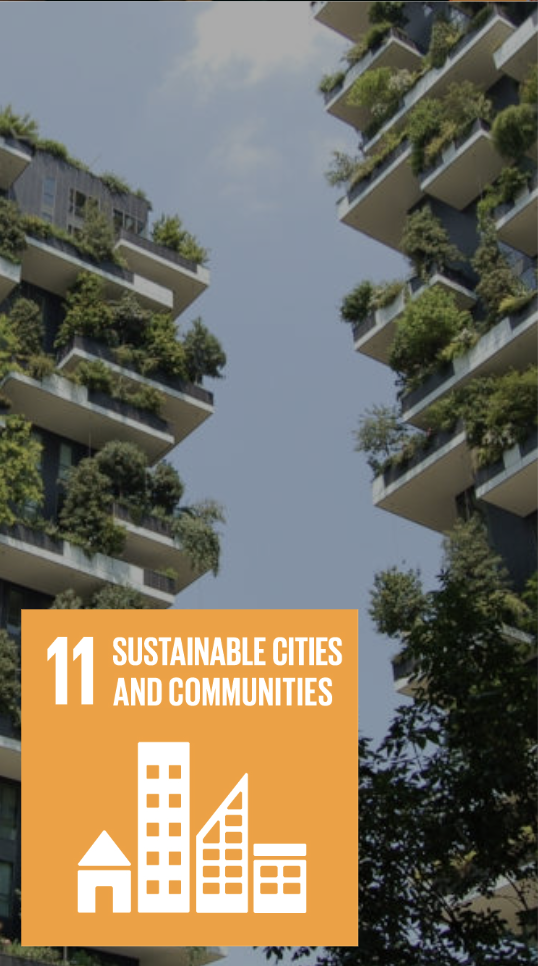
\includegraphics[width=0.48\linewidth,height=\textheight,keepaspectratio]{images/clipboard-1082032997.png}

}

\caption{SDG 11: Sustainable Cities and Communities}

\end{figure}%

From a broader perspective, optimizing heat action plans using
high-resolution spatial data is a key pathway to achieving the United
Nations Sustainable Development Goals. First, this directly contributes
to Goal 11 (Sustainable Cities and Communities) by precisely identifying
surface temperatures to determine how cities can improve infrastructure
and enhance their resilience to climate-related disasters. Second, this
data-driven approach helps reduce health inequalities, aligning with
Goal 3 (Good Health and Well-being), and ensures that marginalized
groups are not left behind during extreme heat waves due to their
disadvantaged geographic locations or economic circumstances. However,
as mentioned earlier, data technology must be integrated with practical
socioeconomic realities to truly realize a sustainable future.

\section{Reflections}\label{reflections}

The results derived from satellite image analysis are free from
subjective bias. They enable decision-makers to quickly bypass the
debate over ``where resources are most needed'' and move directly to the
implementation phase of ``how to carry out interventions.'' Furthermore,
since this data is inexpensive to obtain and updated rapidly, it
significantly reduces the burden on field staff responsible for data
collection.

However, Satellites measure surface temperatures，such as how hot a
rooftop or asphalt road is. This does not equate to the air temperature
or indoor temperature that residents actually experience. An area with
extremely high LST and low NDVI could be a large, modern shopping mall
with central air conditioning. Conversely, an urban village that appears
to be surrounded by greenery may actually consist of shantytowns built
with corrugated iron roofs and extremely poor ventilation, where
residents are enduring deadly indoor heat. Relying solely on ``red
zones'' on satellite imagery to allocate relief supplies can easily lead
to a severe misallocation of resources.

\bookmarksetup{startatroot}

\chapter{Meet Earth Google Engine}\label{meet-earth-google-engine}

\section{Introduction}\label{introduction-2}

Revisiting Google Earth Engine (GEE) this week instantly brought back
memories of my first encounter with this technology during my
undergraduate studies. Back then, I tried using GEE to analyze urban
expansion, and what impressed me most was how convenient it was. Unlike
traditional remote sensing, there was no need to search for data on
official websites, endure lengthy download processes, or consume vast
amounts of local storage. With just a few lines of simple code, I could
directly access massive historical datasets in the cloud for analysis
and instantly render the results in an intuitive, interactive world map
below the editor. It shattered my preconceived notion that remote
sensing software had to process data locally.

\begin{figure}[H]

{\centering \pandocbounded{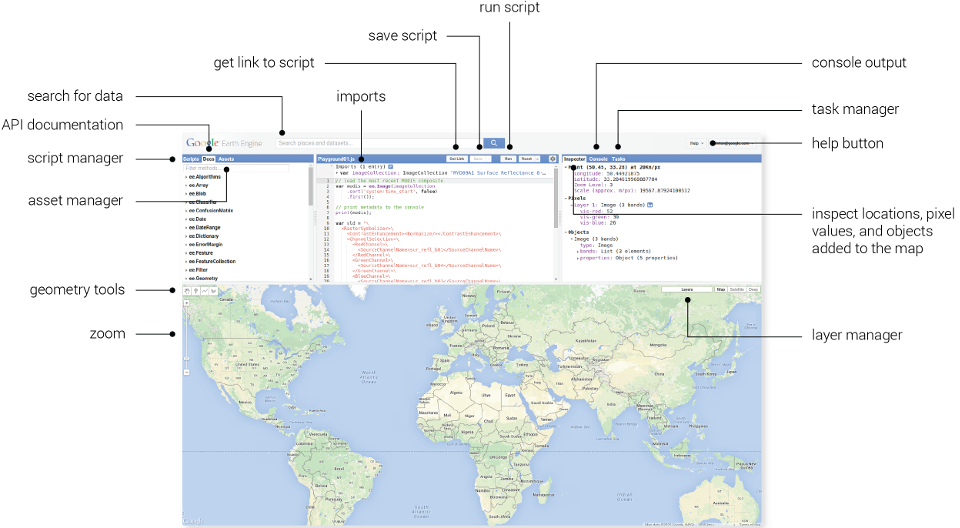
\includegraphics[keepaspectratio]{images/clipboard-3685114081.png}}

}

\caption{Google Earth Engine Code Editor}

\end{figure}%

My favorite part is Google Earth Engine's Data Catalog. Essentially,
it's GEE's official data repository. Basically, it brings together a
wide variety of geospatial data from the 1970s to the present, including
the widely used Landsat and Sentinel satellite imagery, as well as
ready-to-use products such as temperature, precipitation, and land cover
classifications.

\begin{figure}[H]

{\centering \pandocbounded{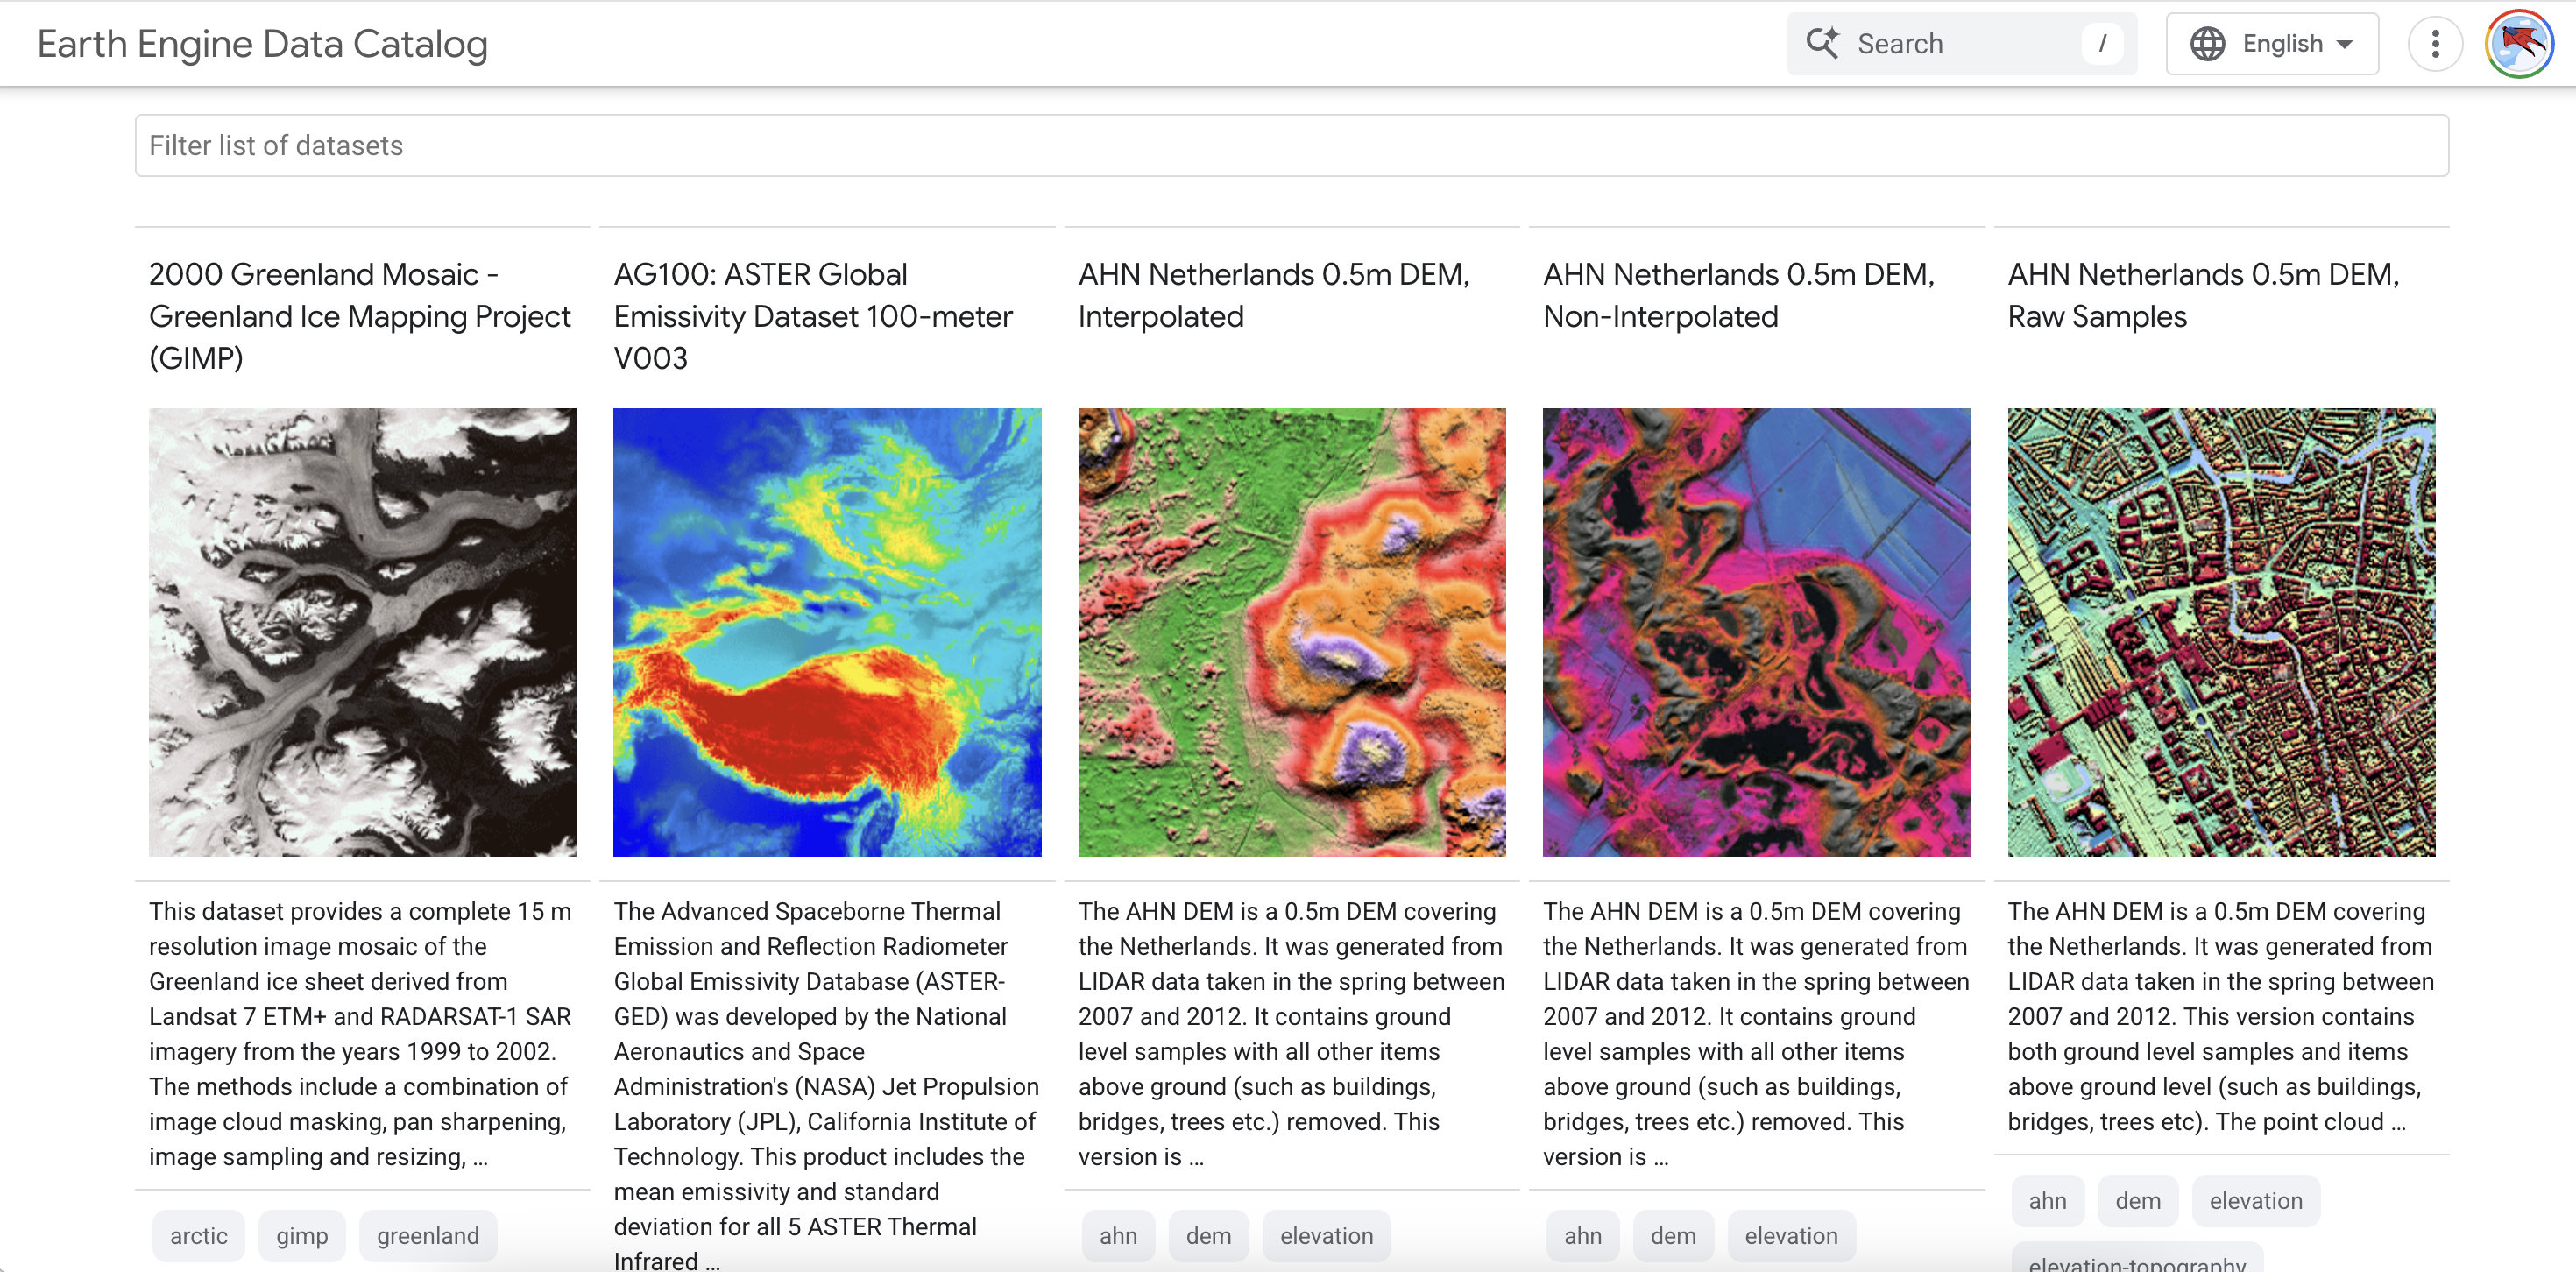
\includegraphics[keepaspectratio]{images/clipboard-2647060660.png}}

}

\caption{Google Earth Engine Catalog Page}

\end{figure}%

It is closely integrated with GEE's actual workflow. After searching for
and selecting a dataset on the Catalog page, you can directly access the
raw data in the cloud for analysis without needing to download any files
yourself. It acts like an online manual, helping you look up band
parameters and view the data's temporal coverage, and allowing you to
jump directly to the programming interface with a single click to get
started.

\section{Application}\label{application-2}

One aspect I found particularly interesting during my studies was the
GEE App. Unlike simply writing code to perform analyses, GEE allows you
to turn the entire analysis process into an interactive web application,
enabling users to view results through a simple interface without
needing to understand the code itself.

I've looked at some existing GEE apps. One that left a particularly
strong impression on me is the Global Forest Change app, which is
primarily used to visualize changes in forest cover and deforestation on
a global scale. It presents what are typically complex remote sensing
analysis results in a very intuitive way---for example, using red to
indicate forest loss and green to indicate existing forests---so that
even users without prior background knowledge can quickly understand the
data. Additionally, it makes excellent use of time-series data, allowing
users to view changes over multiple years rather than just at a single
point in time.

\begin{figure}[H]

{\centering \pandocbounded{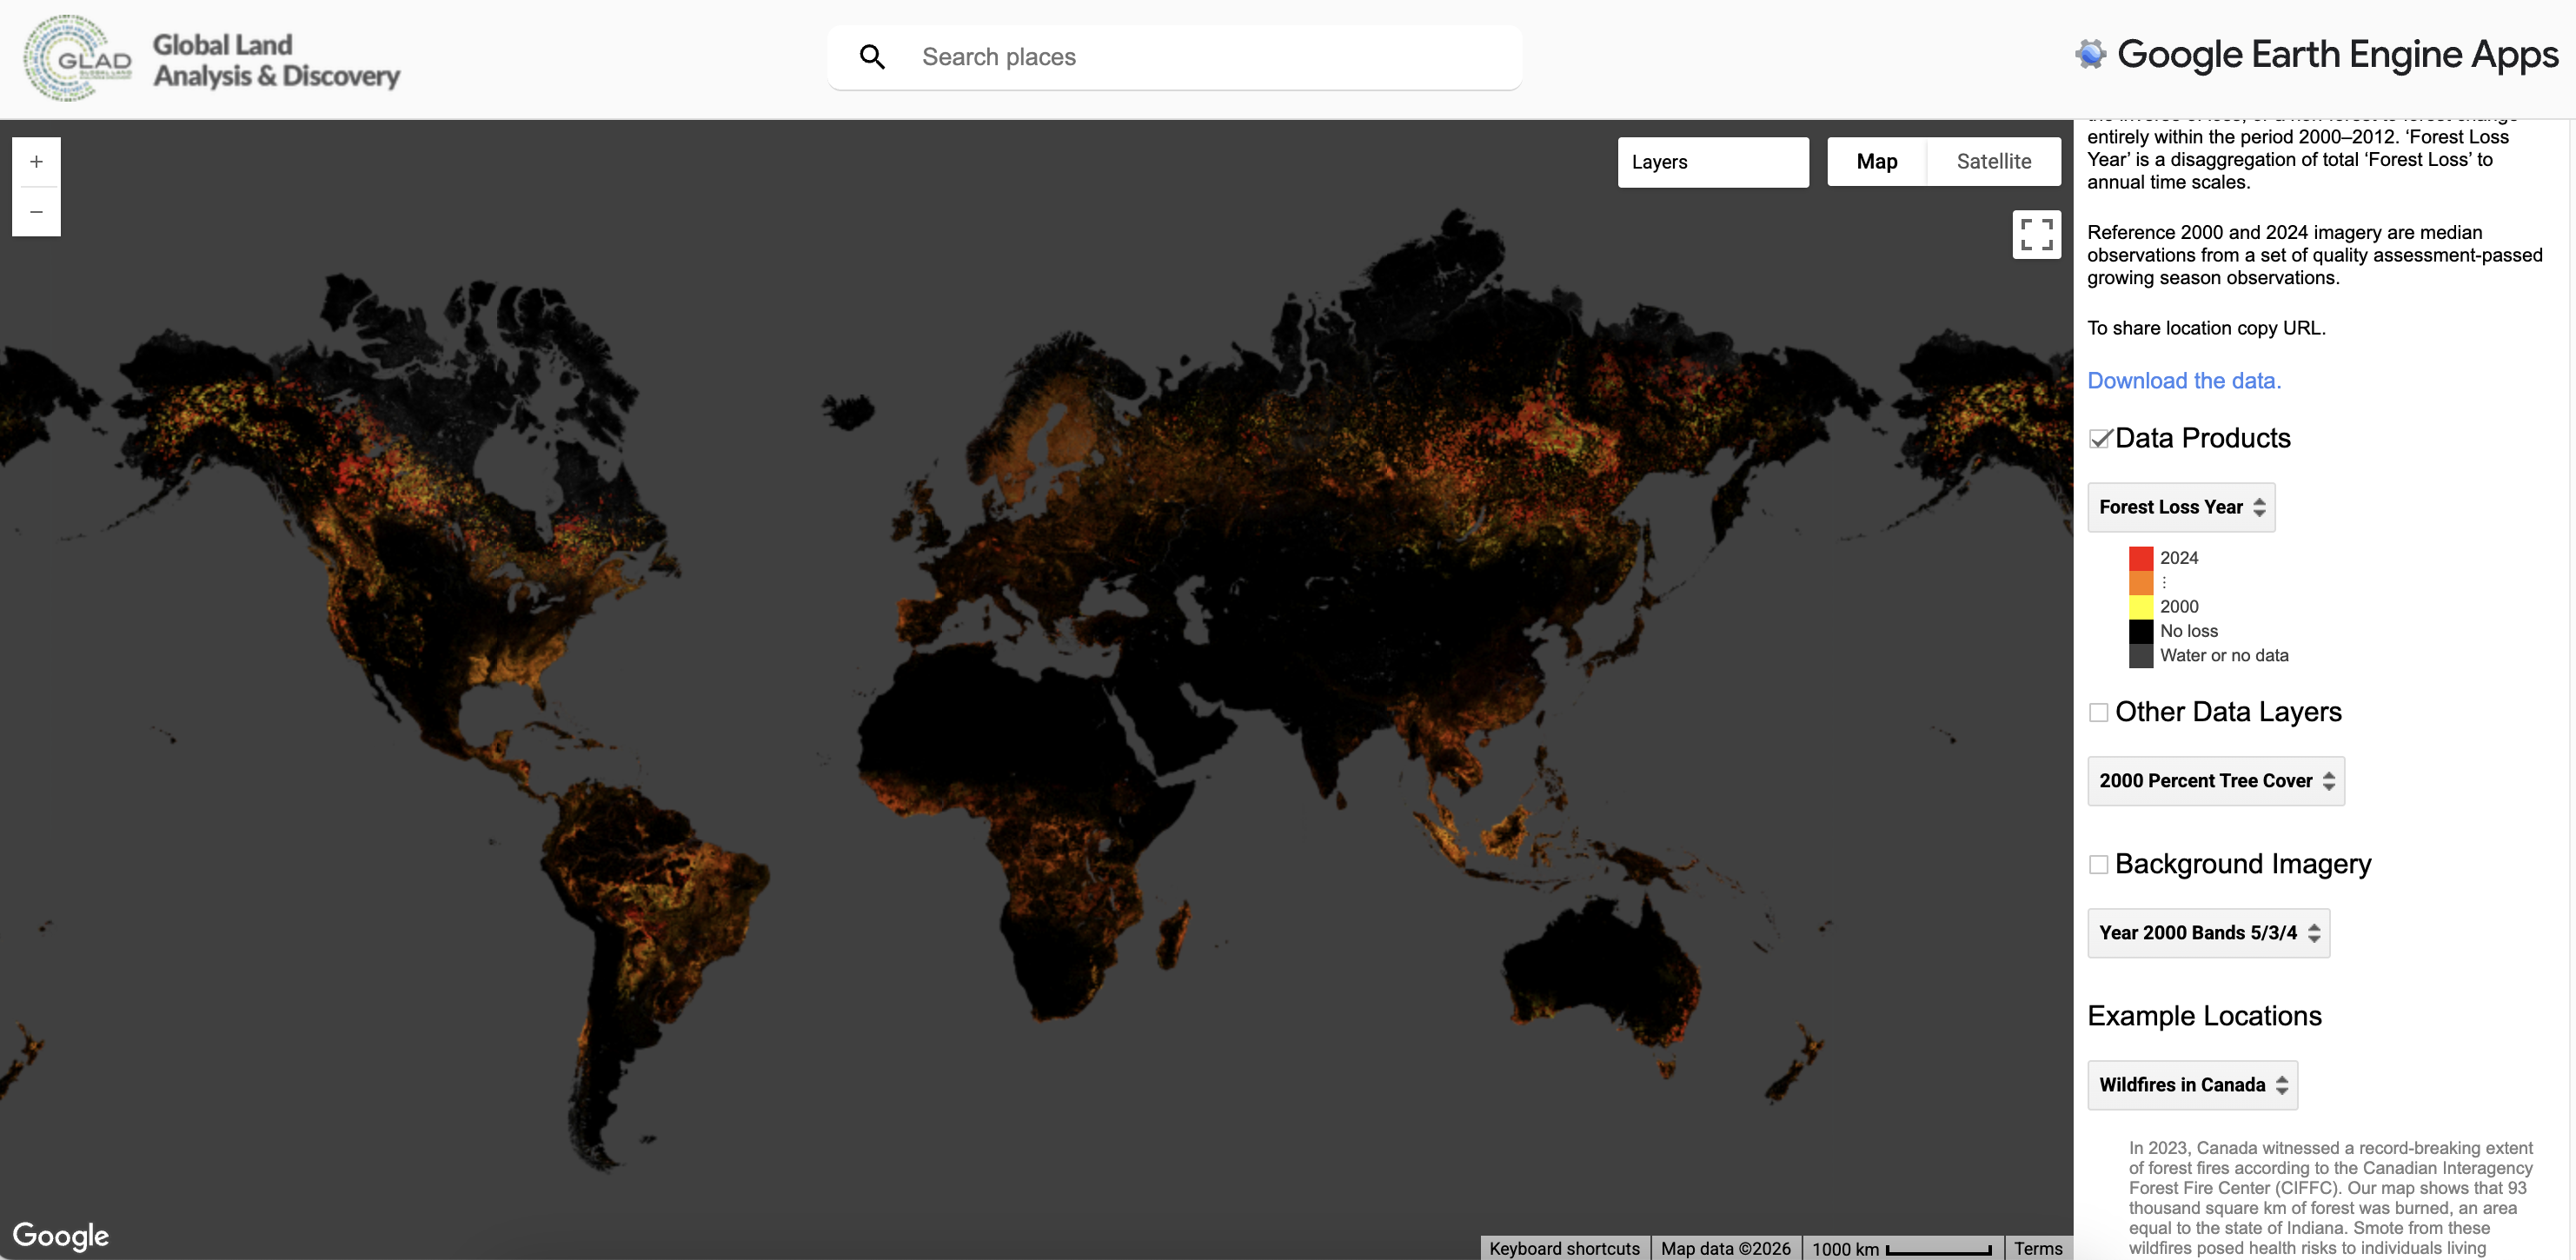
\includegraphics[keepaspectratio]{images/clipboard-1817680799.png}}

}

\caption{Global Forest Change app}

\end{figure}%

If you'd like to learn more, watch the video below for a clearer
understanding of the GEE App's design and applications.

\url{https://www.youtube.com/watch?v=EJFYEaYeL4o}

\section{Reflection}\label{reflection-2}

To be honest, after working with GEE this week, my biggest takeaway is
that I probably never want to go back to the old way of working with
traditional software like ArcGIS or ENVI. With those traditional
software tools, I had to remember complicated steps every time I ran a
process. Clicking the right icon, entering the correct parameters. If
you clicked the wrong button or wanted to change a parameter, you'd
almost have to start from scratch. Writing code in GEE might be a bit
overwhelming at first, but it's truly ideal for processing large volumes
of files, and you can open and run it directly later on. I can modify
any step in the workflow, and the entire process is crystal clear and
fully reproducible.

However, GEE is definitely not perfect, and I've run into a few
frustrating hurdles in the past.

\begin{itemize}
\item
  The computational performance isn't very strong. As soon as you try to
  process images that are slightly larger or have higher resolution, the
  progress bar moves extremely slowly. I often find myself staring at
  the screen for ages, only to end up with a ``Computation timed out''
  error.
\item
  Its preprocessing workflow is somewhat of a ``black box.'' While it's
  convenient to receive fully processed data, this also means we lose
  the ability to choose different preprocessing methods (such as
  atmospheric correction or terrain correction algorithms).
\item
  What frustrates me the most is its debugging mechanism. In RStudio or
  VS Code, we can test code in blocks, but with GEE, you almost always
  have to run the entire script from start to finish. If an error occurs
  midway through, it's difficult to determine whether the problem lies
  in the code logic or if the cloud server itself has stalled. I find
  this approach extremely time-consuming.
\end{itemize}

\bookmarksetup{startatroot}

\chapter{Classification 1}\label{classification-1}

\section{Summary}\label{summary-2}

After learning the basics of GEE last week, this week's topic is
classification using machine learning. I realized that the
``classification'' tools I used to work with in ENVI or ArcGIS were
actually based on supervised learning. In our introductory courses, we
simply referred to them as ``image classification.'' It wasn't until
this week that I truly understood the logic behind these tools.

Why do we perform image classification? Satellite image data consists of
nothing more than pixels with numerical values. Our goal is to transform
these meaningless numbers into ``semantic information'' that humans can
understand, such as identifying where buildings are located and where
bodies of water are found. We use remote sensing techniques to quantify
urban sprawl, deforestation, and environmental changes.

The core of image classification lies in the use of spectral signatures.
Different land features exhibit vastly different reflectance across
different spectral bands. The classifier's task is to learn the patterns
of these spectral characteristics by analyzing the training samples we
provide.Then, automatically classify the pixels across the entire map.

\begin{longtable}[]{@{}
  >{\raggedright\arraybackslash}p{(\linewidth - 8\tabcolsep) * \real{0.2000}}
  >{\raggedright\arraybackslash}p{(\linewidth - 8\tabcolsep) * \real{0.2000}}
  >{\raggedright\arraybackslash}p{(\linewidth - 8\tabcolsep) * \real{0.2000}}
  >{\raggedright\arraybackslash}p{(\linewidth - 8\tabcolsep) * \real{0.2000}}
  >{\raggedright\arraybackslash}p{(\linewidth - 8\tabcolsep) * \real{0.2000}}@{}}
\toprule\noalign{}
\begin{minipage}[b]{\linewidth}\raggedright
Aspect
\end{minipage} & \begin{minipage}[b]{\linewidth}\raggedright
CART
\end{minipage} & \begin{minipage}[b]{\linewidth}\raggedright
Random Forest
\end{minipage} & \begin{minipage}[b]{\linewidth}\raggedright
Naive Bayes
\end{minipage} & \begin{minipage}[b]{\linewidth}\raggedright
SVM
\end{minipage} \\
\midrule\noalign{}
\endhead
\bottomrule\noalign{}
\endlastfoot
Core Idea & Recursive splitting & Ensemble voting & Probabilistic model
& Max margin separation \\
Overfitting & High & Low & Low & Medium \\
Training Speed & Fast & Medium & Very fast & Slow \\
Interpretability & High & Low & Medium & Low \\
Best Use Cases & Simple rules & General tasks & Text classification &
High-dim data \\
\end{longtable}

Since Xinjiang in China encompasses a wide variety of landforms. I
initially worked with a Level 1 region. However, GEE quickly froze and
returned an error due to the massive computational load. So I promptly
narrowed the scope down to Beijing. I used the QA60(specifically records
whether each pixel is covered by opaque clouds or cirrus clouds.) band
to remove areas with cloud cover and calculated the median of the
remaining images for the year, resulting in a clean base map.

I don't have a large number of sample areas, so to improve
classification accuracy, I generated 1,000 random points within each
ground-truth patch. This helps prevent overfitting caused by a lack of
diversity in the samples.

\begin{figure}[H]

{\centering 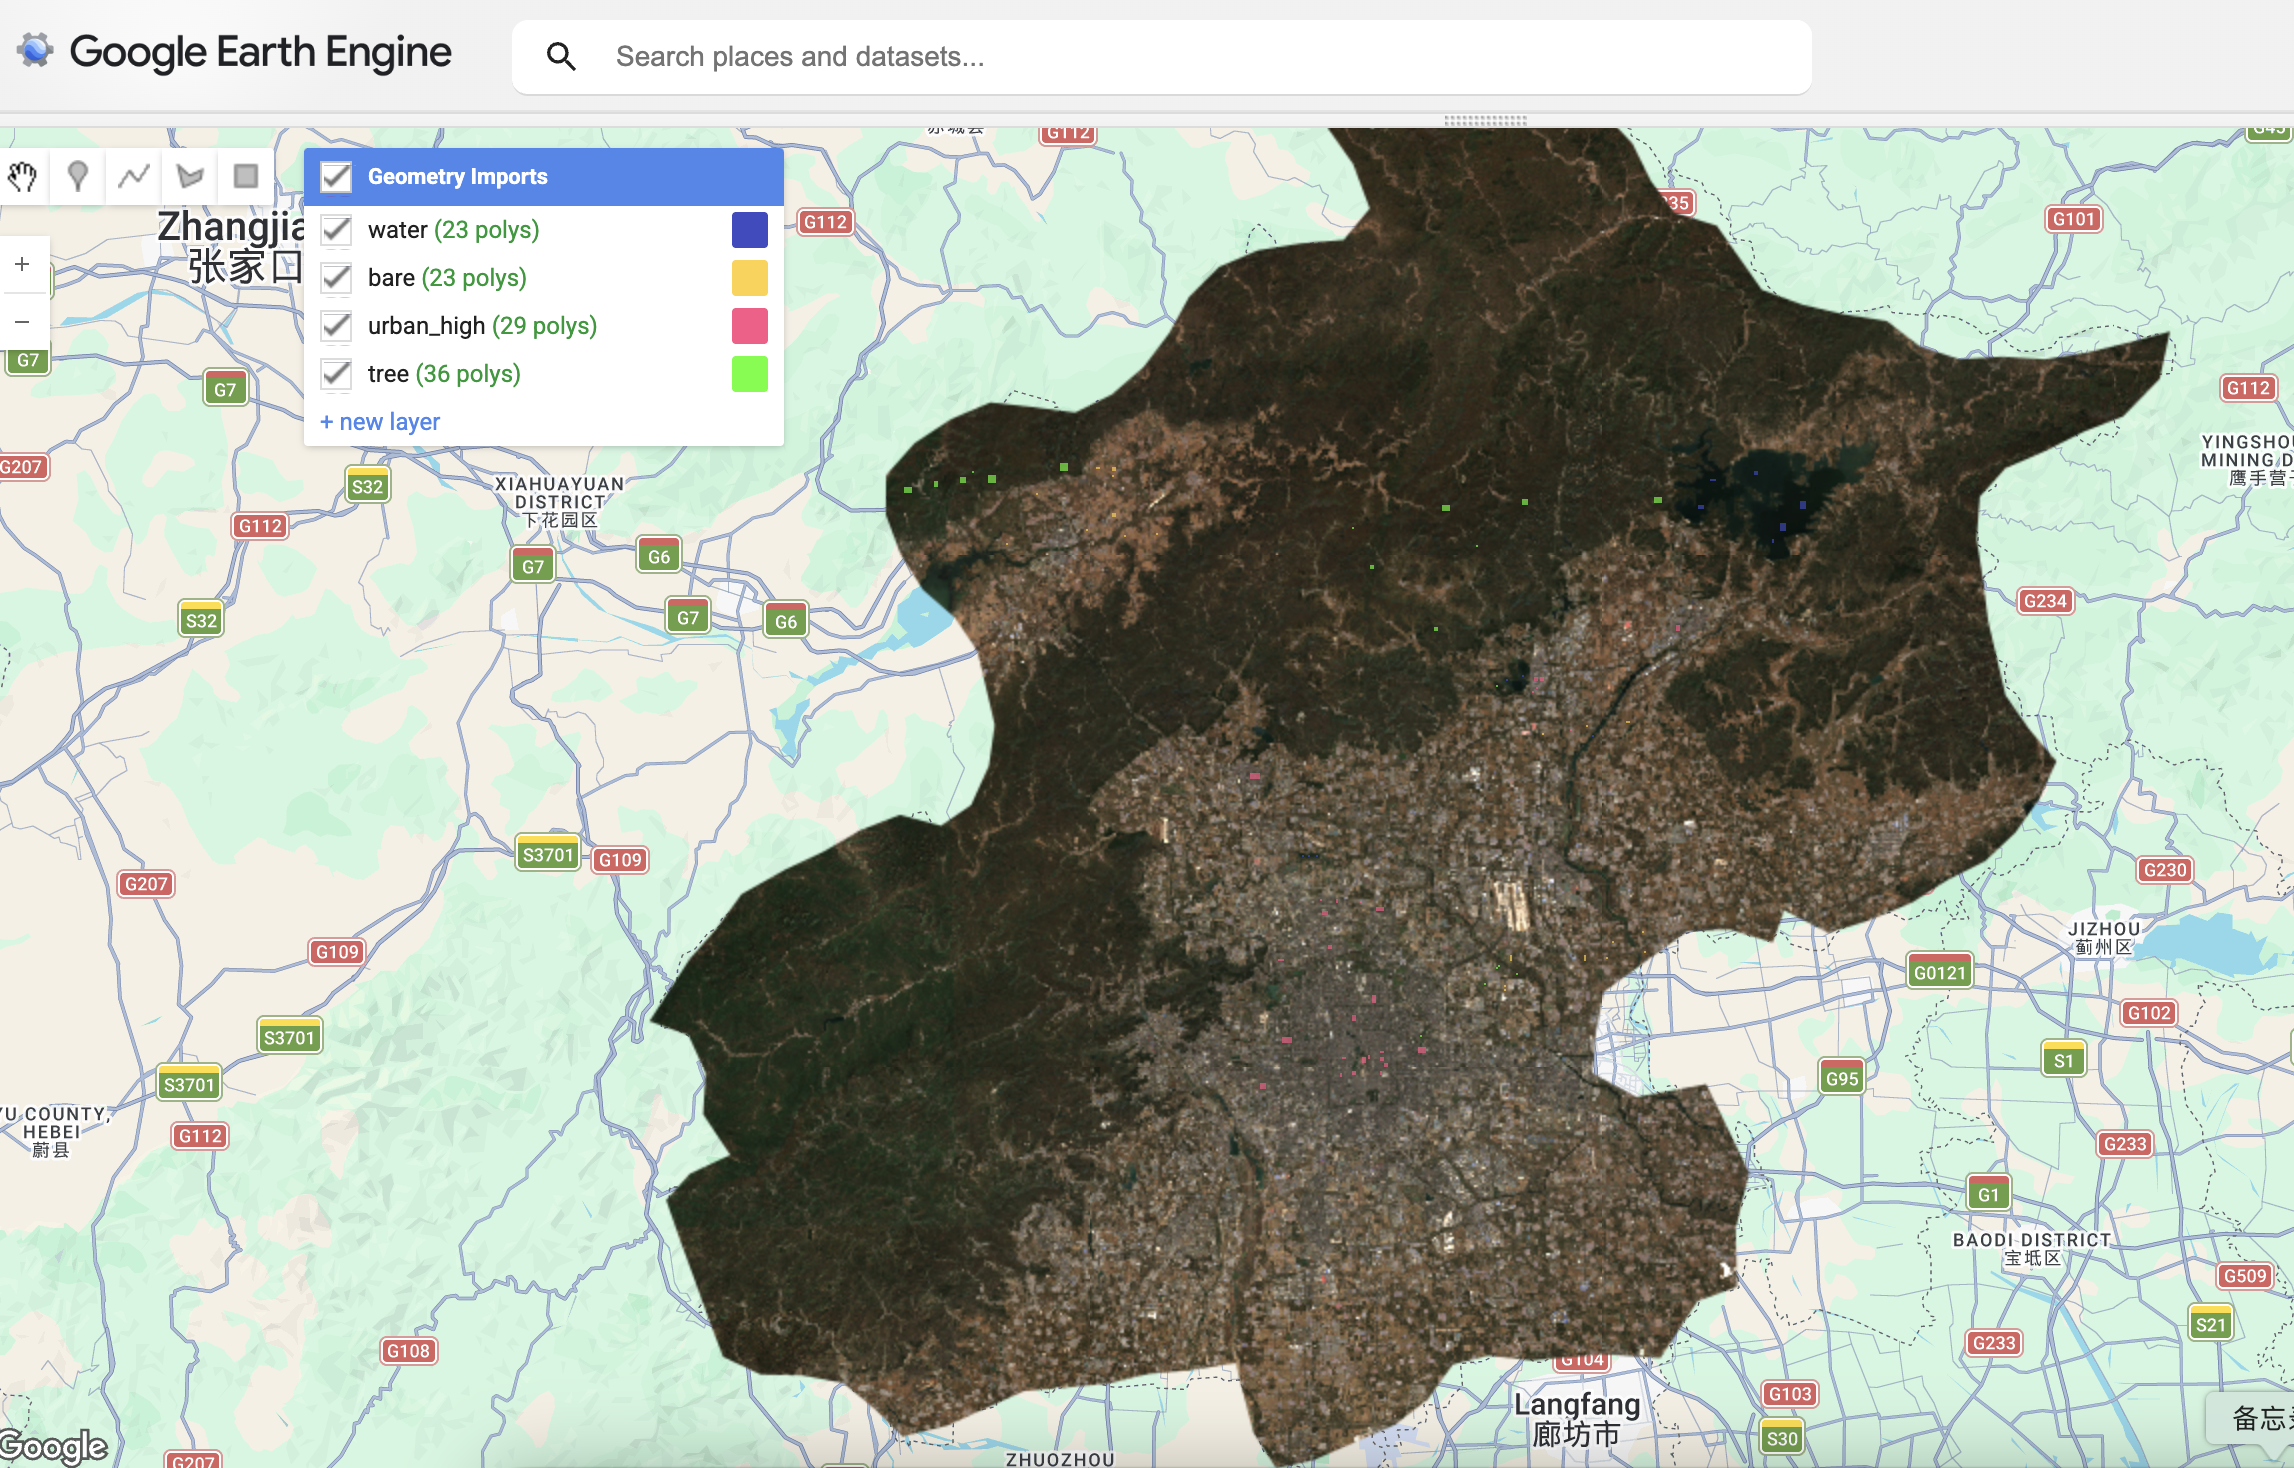
\includegraphics[width=5.09375in,height=\textheight,keepaspectratio]{images/clipboard-3990678885.png}

}

\caption{Beijing Training Polygons}

\end{figure}%

I selected a total of nine bands, specifically including the two
short-wave infrared bands, B11 and B12. These are particularly effective
for distinguishing between urban buildings in Beijing and the
surrounding hillsides and wasteland(Jocea et al. 2025).

During the experiment, I ran two algorithms: CART and Random Forest.

\begin{figure}[H]

{\centering 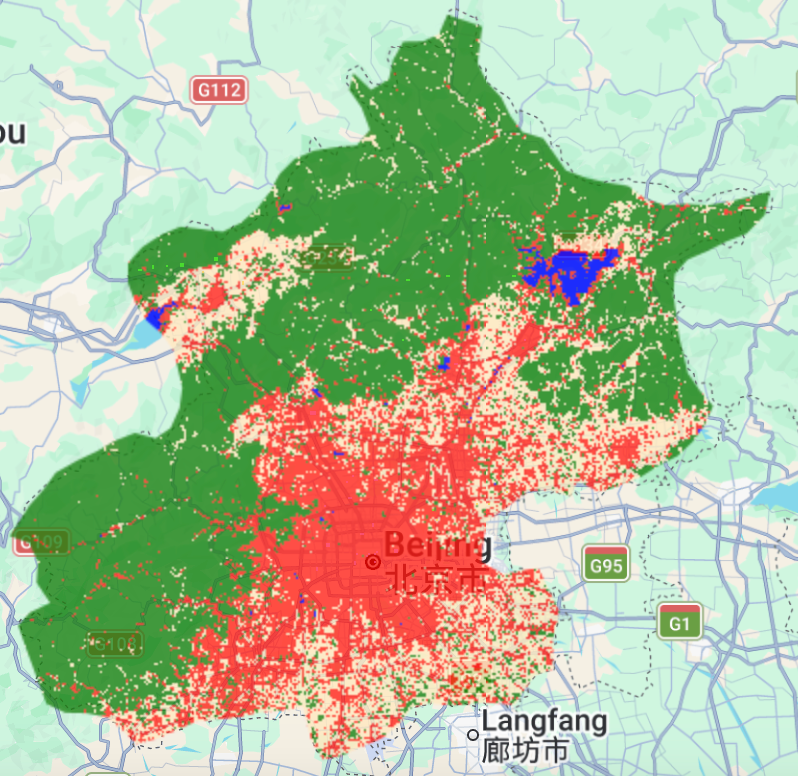
\includegraphics[width=3.89583in,height=\textheight,keepaspectratio]{images/clipboard-570344990.png}

}

\caption{CART category results}

\end{figure}%

\textbf{Random Forest} is known for its stability. To properly validate
the model, I kept 30\% of the data hidden during training to use for a
final test. The results were actually quite good, with a validation
accuracy of 0.969. The final confusion matrix shows that the
classification accuracy for water and forest is nearly perfect, while
the primary minor errors are concentrated between urban and bare land.
This is because, in the suburbs of Beijing, the spectral characteristics
of certain building materials are highly similar to those of soil.

\begin{figure}[H]

{\centering \pandocbounded{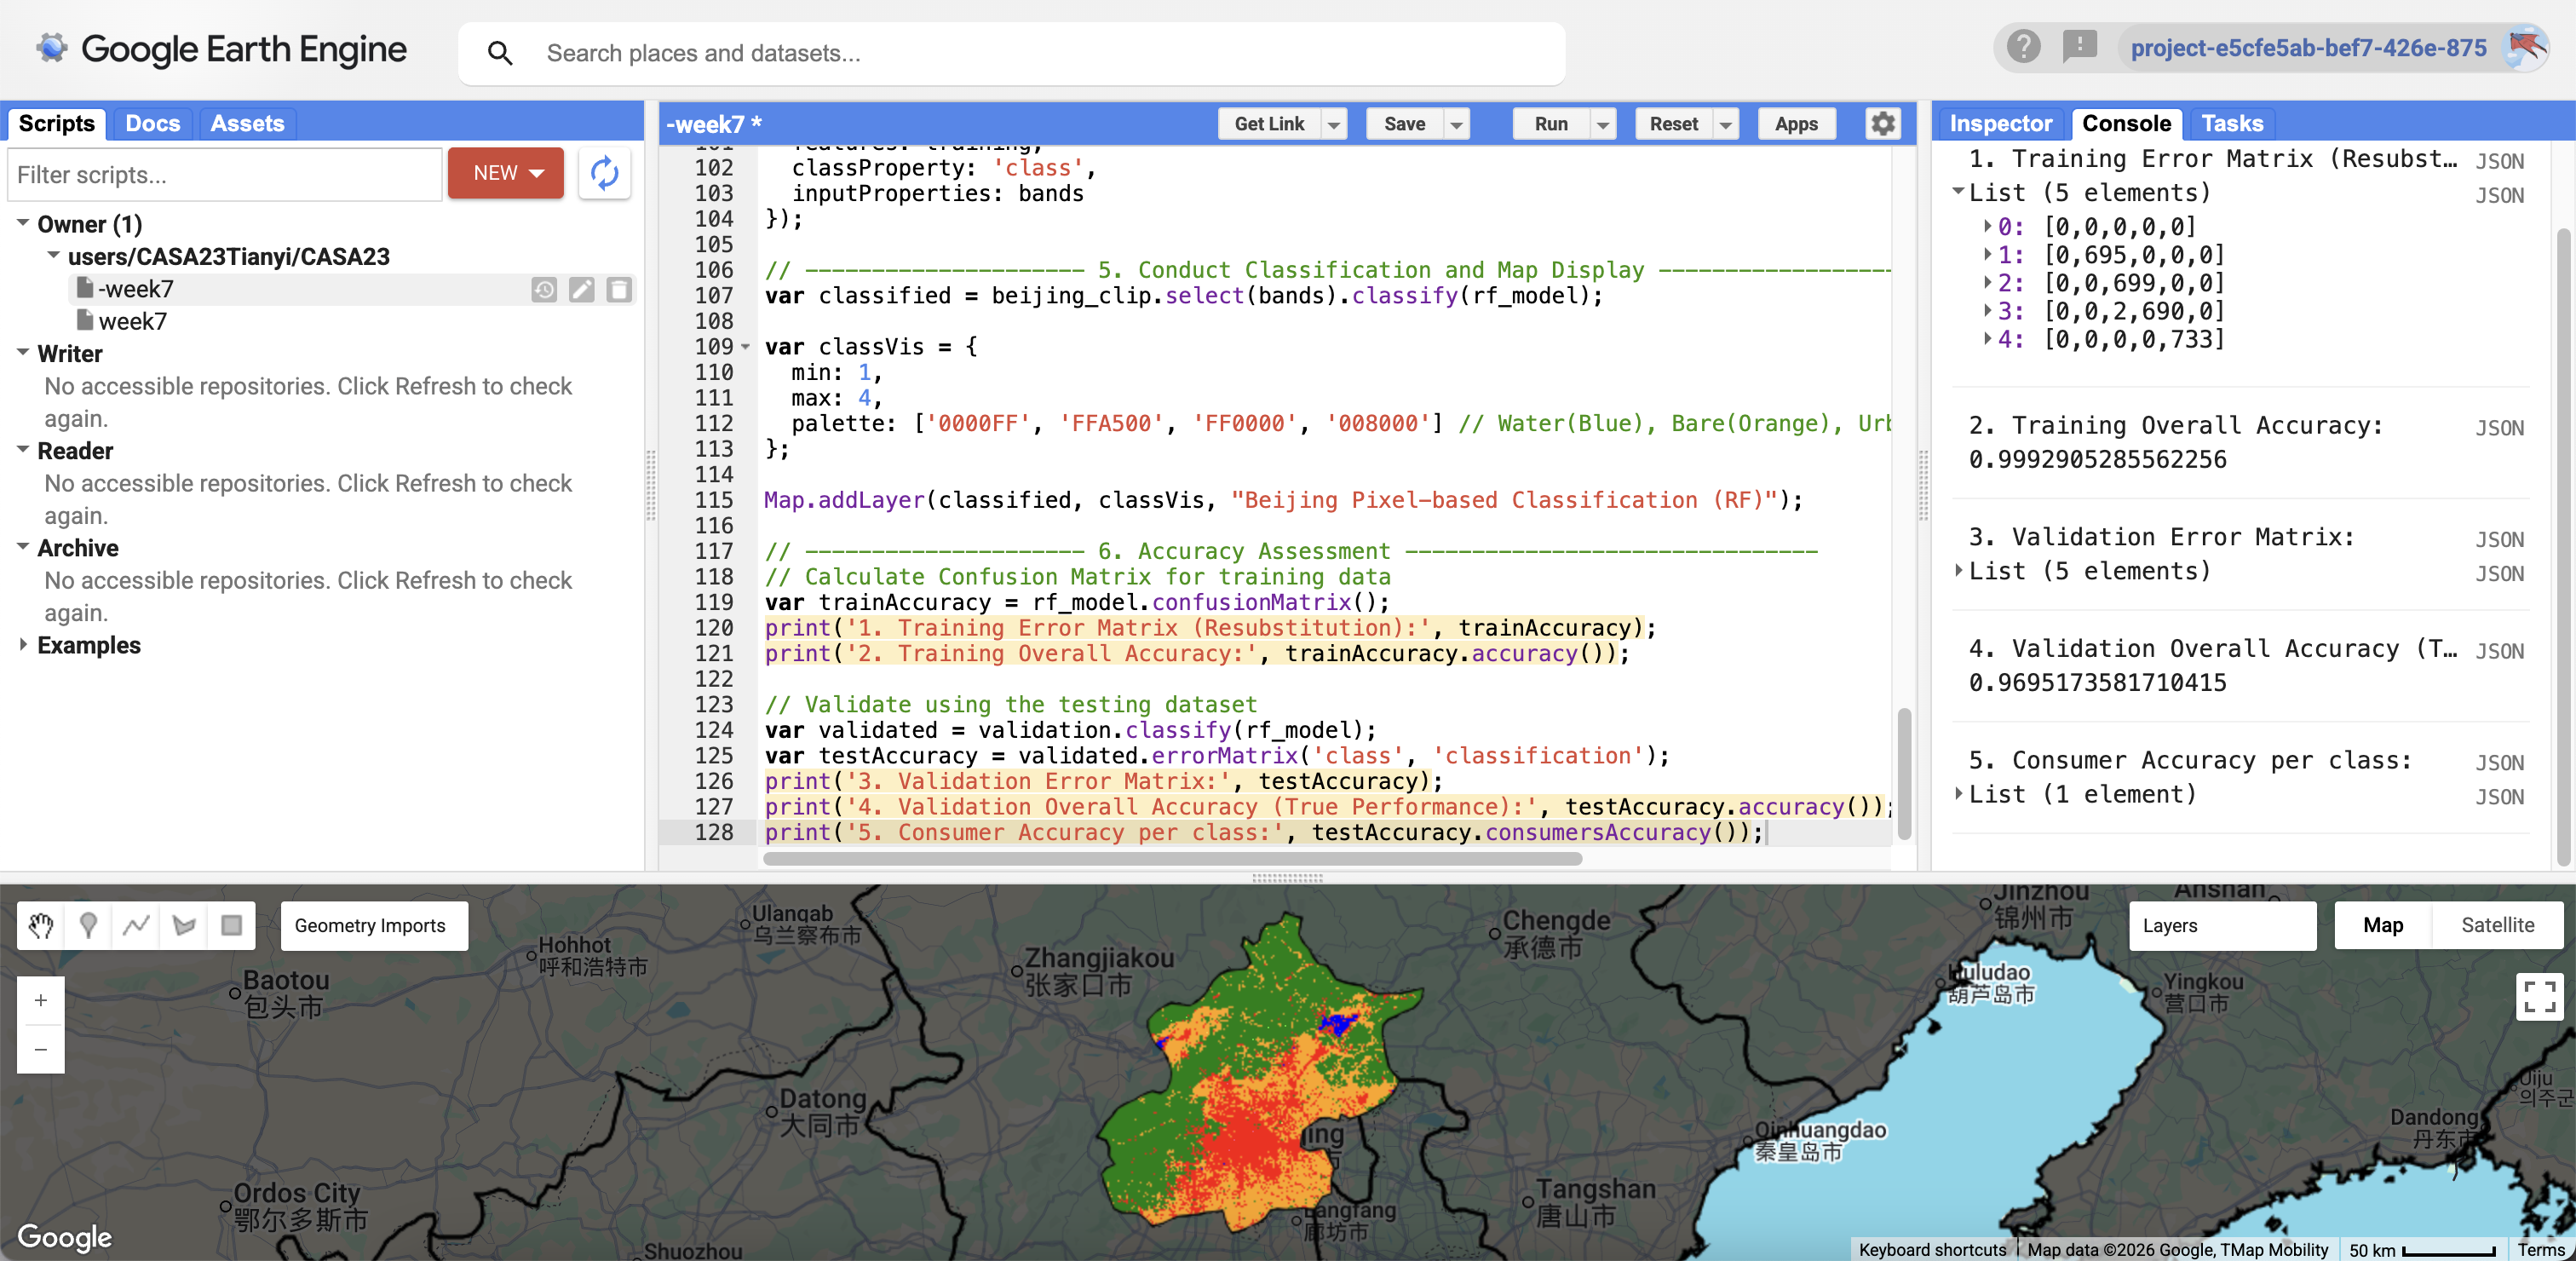
\includegraphics[keepaspectratio]{images/clipboard-1353034869.png}}

}

\caption{Random Forest category results}

\end{figure}%

\section{Applications}\label{applications-1}

Existing research generally indicates that Random Forests typically
outperform CART in terms of classification accuracy and model stability.
For example, (Jocea et al. 2025) shows that the overall accuracy of
Random Forests can reach 0.96--0.98, whereas CART's accuracy is
relatively lower and more volatile.

This difference in performance can be attributed to differences in model
architecture. CART is a single decision tree model that is susceptible
to the training data and prone to overfitting(Leo Breiman et al. 1984).
In contrast, Random Forests effectively reduce model variance by
aggregating the predictions of multiple decision trees through voting,
resulting in high generalization ability(L. Breiman 2001).

However, it is important to note that CART is not totally inferior to
Random Forests. If the data structure is relatively simple or the
differences between classes are distinct, CART can still achieve good
classification results. Furthermore, CART offers good interpretability
and retains an advantage in certain application scenarios where an
explanation of the model's decision-making process is required.

Although the Random Forest algorithm was first proposed as early as 2001
and has undergone more than two decades of development, what changes and
improvements have been made?

\begin{figure}[H]

{\centering 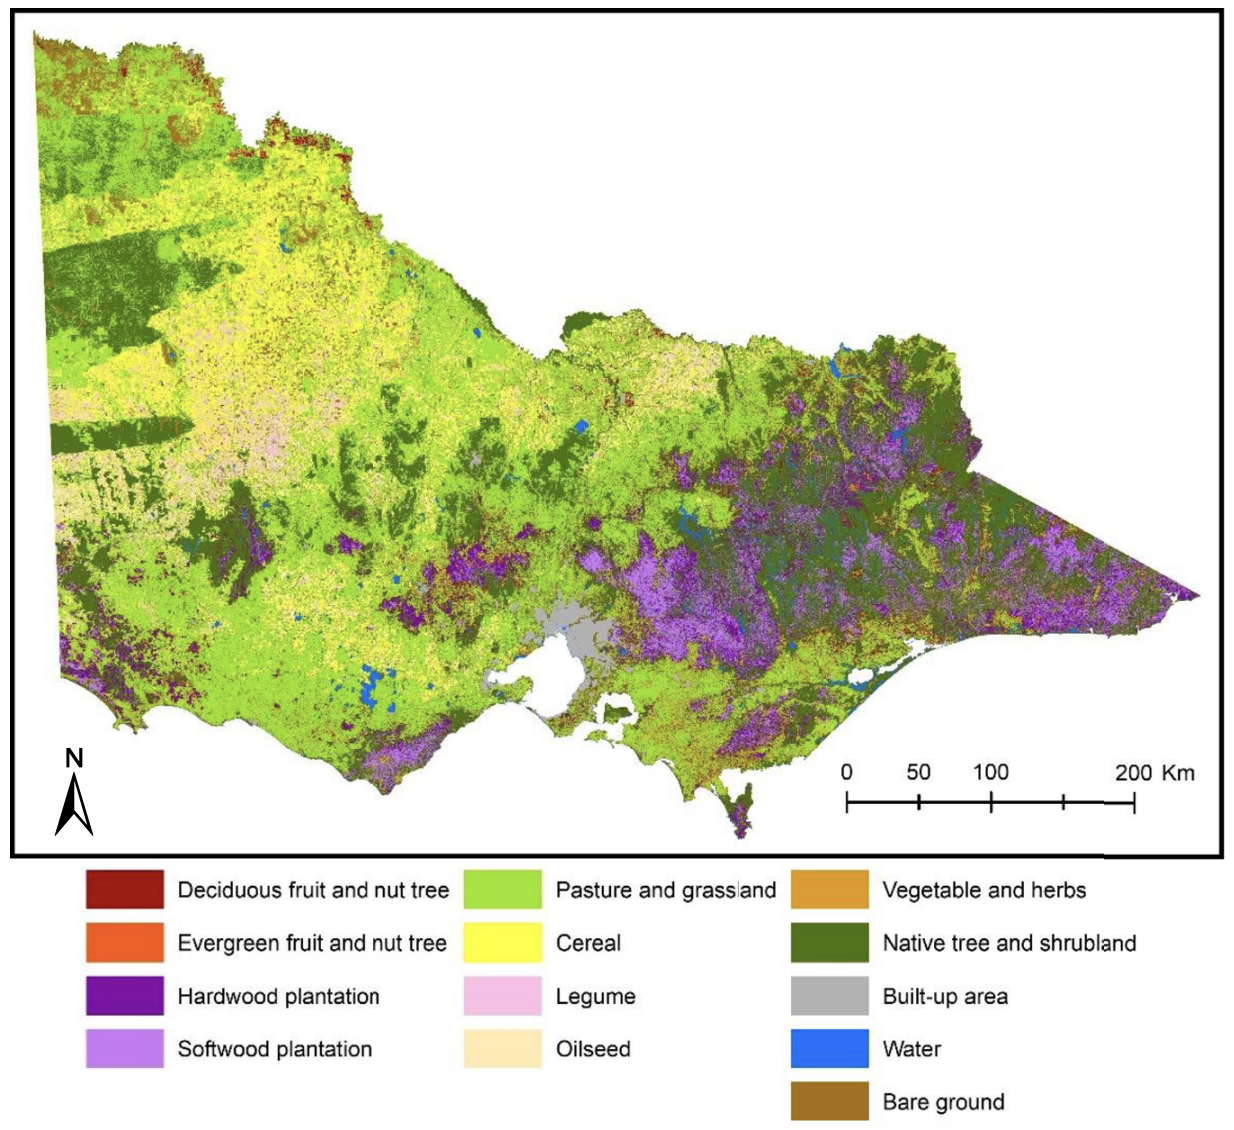
\includegraphics[width=5.96875in,height=\textheight,keepaspectratio]{images/clipboard-635645688.png}

}

\caption{Land cover map across the Victoria state at 20m spatial
resolution for 2021/22.(Sabaghy et al. 2025)}

\end{figure}%

The increasing accessibility of high-resolution Sentinel-2 and UAV
imagery has shifted the research focus toward finer-scale features and
intricate land cover types. Rather than relying solely on spectral data,
modern approaches now integrate multiple sources---including textural
and topographic information---while optimizing parameters to boost both
accuracy and model stability. Consequently, the field has evolved from
broad macro-scale mapping in agriculture to specialized applications
like urban land-use classification(Sabaghy et al. 2025), wetland
conservation, and real-time disaster monitoring.

\section{Reflection}\label{reflection-3}

In this week's training, the number of hand-drawn polygons was limited,
with only about a dozen for each category, making it difficult for the
model to fully learn the spectral characteristics of objects. Although
pixel-level random sampling increased the sample size and improved model
accuracy, it may have led to a concentration of training samples in
certain areas, failing to fully reflect regional heterogeneity. In the
future, we may consider more uniform or stratified sampling.

During the classification process, spectral similarities between
buildings and bare ground led to some confusion, highlighting the
limitations of relying solely on spectral bands for classification. In
the future, category discrimination could be improved by incorporating
texture features or the Normalized Difference Building Index (NDBI). In
complex urban environments, spectral information may not be sufficient
to resolve all classification challenges; therefore, future research
should explore methods that combine spatial structural features with
multi-temporal data.

While reviewing the literature, I noticed a cutting-edge trend of
combining random forests with predictive models. For example, the paper
``Simulation of Wetland Changes in the Wuhan Urban Agglomeration Based
on the Integration of Random Forests and the CLUE-S Model'' demonstrates
how to use machine learning to extract features and couple them with
spatial models for multi-scenario simulations(Peng et al. 2020). This
gives me a new idea: I could use the current Beijing classification as
baseline, add models like CLUE-S or CA-Markov, and combine population
and traffic data to simulate future land cover changes.

\bookmarksetup{startatroot}

\chapter{Classification 2}\label{classification-2}

\section{Summary}\label{summary-3}

This week marks a transition from basic pixel-based classification
towards more advanced approaches in remote sensing, prompting me to
rethink the role of the pixel as the fundamental spatial unit. In
previous weeks, classification methods largely followed a simplified
assumption that each pixel can be assigned to a single, discrete land
cover class. While this ``black-and-white'' approach is methodologically
straightforward, it becomes increasingly problematic in complex urban
environments, often leading to biased area estimates.

This week, we explored two advanced approaches for handling complex
ground-level environments:

\begin{itemize}
\item
  \textbf{Sub-pixel unmixing}, which introduces the concept of ``gray
  zones'' to account for spectral mixing within pixels and calculate
  component ratios.
\item
  \textbf{Object-based image analysis}, which breaks down the isolation
  of pixels in the spatial dimension by aggregating adjacent pixels into
  ``superpixel'' objects with shape and texture. This shift from
  ``single labels'' to ``component ratios'' and ``spatially semantic
  objects''.
\end{itemize}

The preprocessing stage already required contextual adjustment. Using
Landsat 8 (L2) imagery, I relaxed the cloud filtering threshold from 1\%
to 5\% to account for Beijing's atmospheric conditions, followed by
cloud masking and median compositing. This highlighted an early
trade-off between data quality and data availability, which inevitably
influences the reliability of downstream classification results.

\subsection{Sub-pixel Analysis}\label{sub-pixel-analysis}

Using the sub-pixel approach gives us a much more flexible way to look
at Beijing's mixed-up urban surface. Basically, we set up some basic
categories, like buildings, water, bare dirt, and trees. Then, instead
of just slapping a single label on a pixel, the model figures out the
exact percentage of each thing inside it.

\phantomsection\label{fancy-layout}
\phantomsection\label{first-pic}
\begin{figure}[H]

{\centering 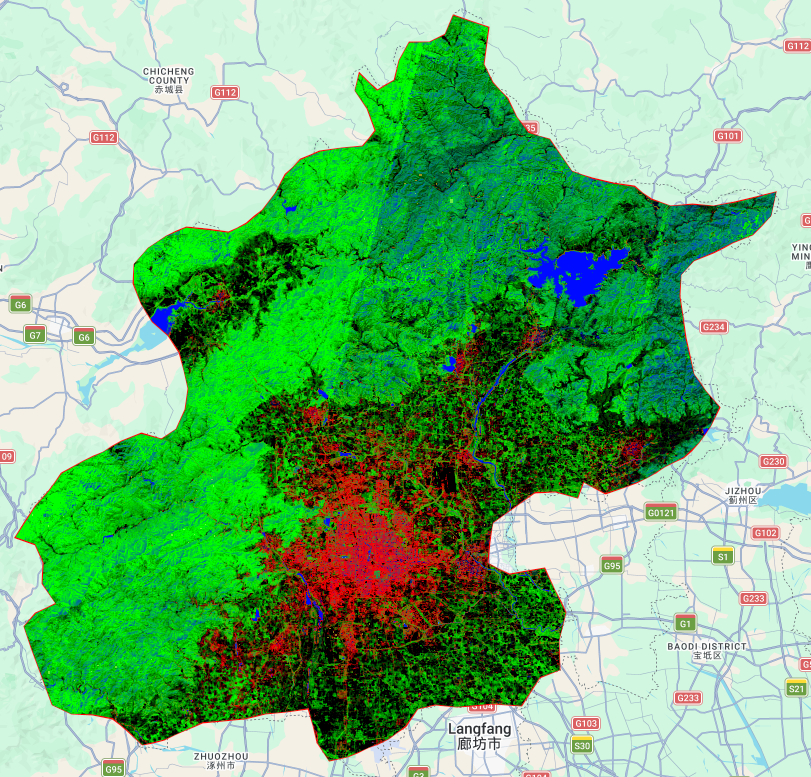
\includegraphics[width=1\linewidth,height=\textheight,keepaspectratio]{images/clipboard-1093845086.png}

}

\caption{Endmember Abundance Composite Map}

\end{figure}%

\phantomsection\label{second-pic}
\begin{figure}[H]

{\centering 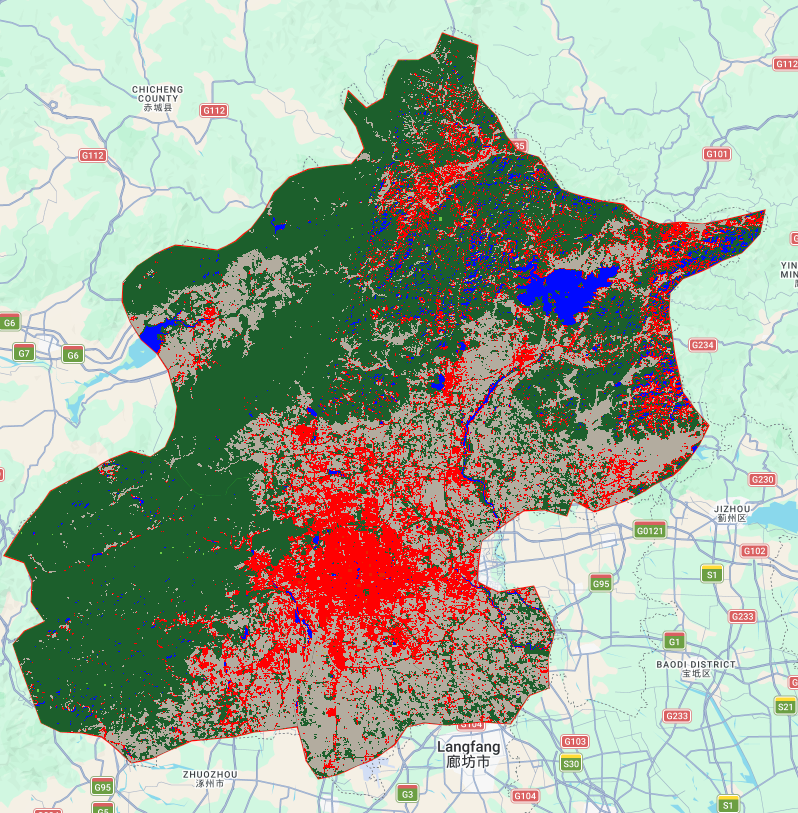
\includegraphics[width=0.93\linewidth,height=\textheight,keepaspectratio]{images/clipboard-3778352811.png}

}

\caption{Threshold-based Land Cover Map}

\end{figure}%

But there's a catch: to actually make sense of the final map and check
its accuracy, we have to force those percentages into fixed, single
categories. And that's its biggest downside. Even though the percentage
idea is way closer to real life, a lot of those subtle details get
totally lost the moment we force them into strict boxes.

\begin{figure}[H]

{\centering \pandocbounded{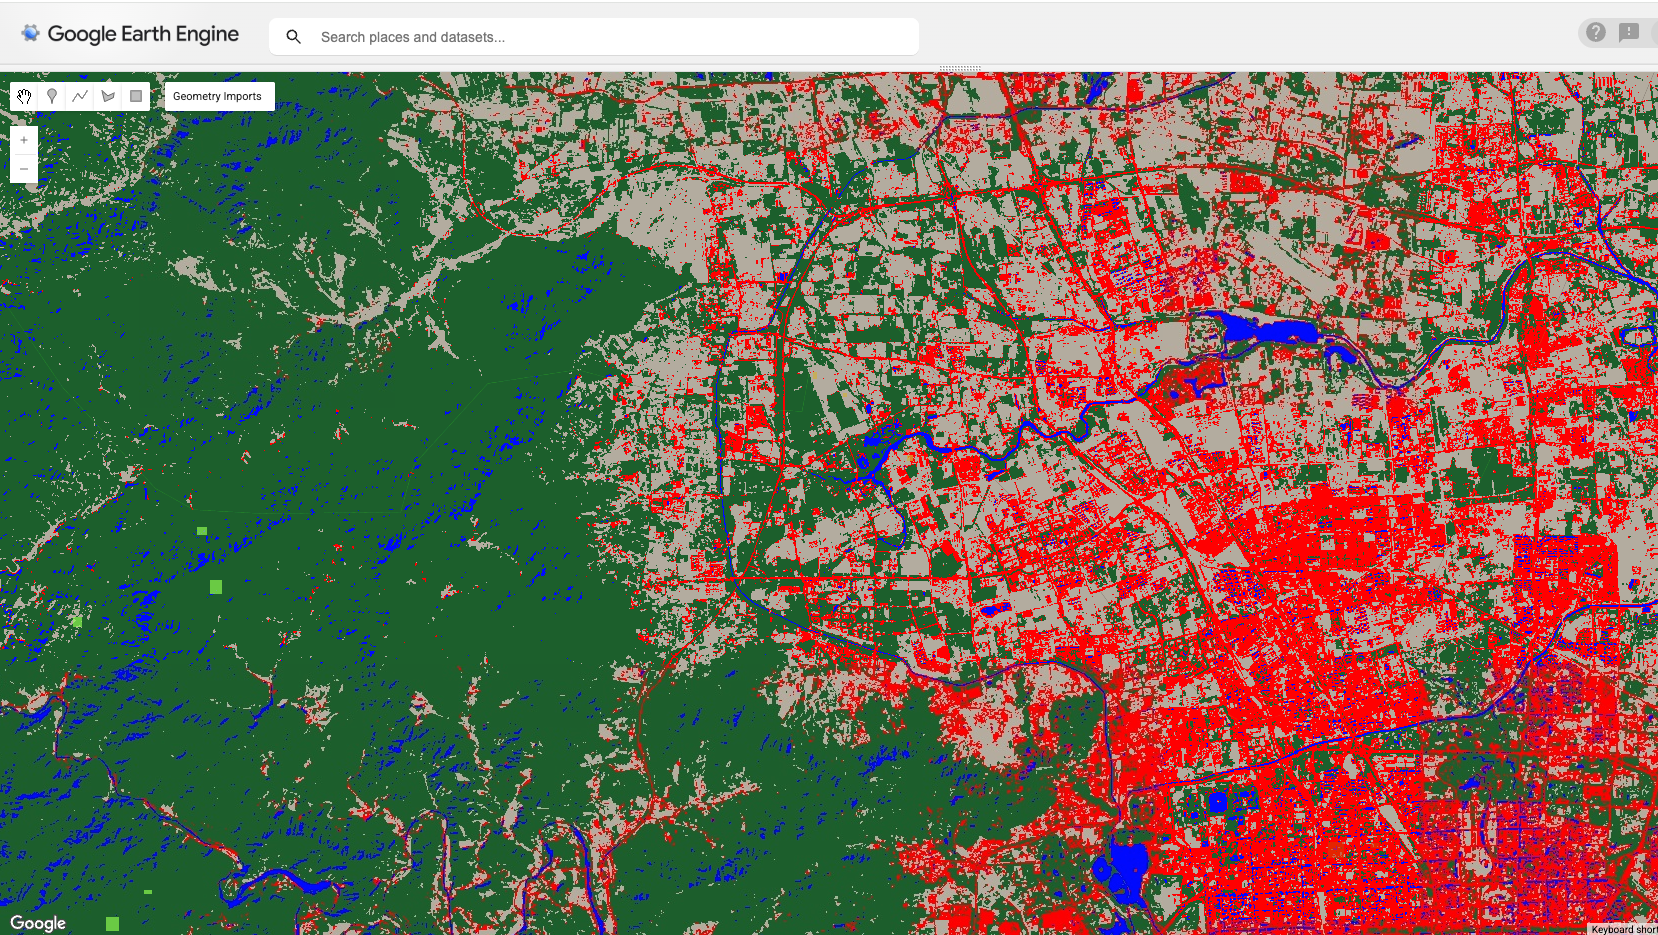
\includegraphics[keepaspectratio]{images/clipboard-4075946674.png}}

}

\caption{Threshold-based Land Cover Map}

\end{figure}%

\subsection{Object-based Image
Analysis}\label{object-based-image-analysis}

The OBIA method makes things look more connected by grouping pixels into
bigger chunks and looking at their texture. Sure, this cleans up the
noise and makes the edges sharper, but in my case, the chunks ended up a
bit too clunky. They formed big blocks that hid a lot of the smaller
details. This just goes to show that OBIA is super picky about its
settings (like how big or tight the chunks are). If you don't tweak it
just right, it struggles to catch the fine details you need for a
complicated city like Beijing.

\begin{figure}[H]

{\centering 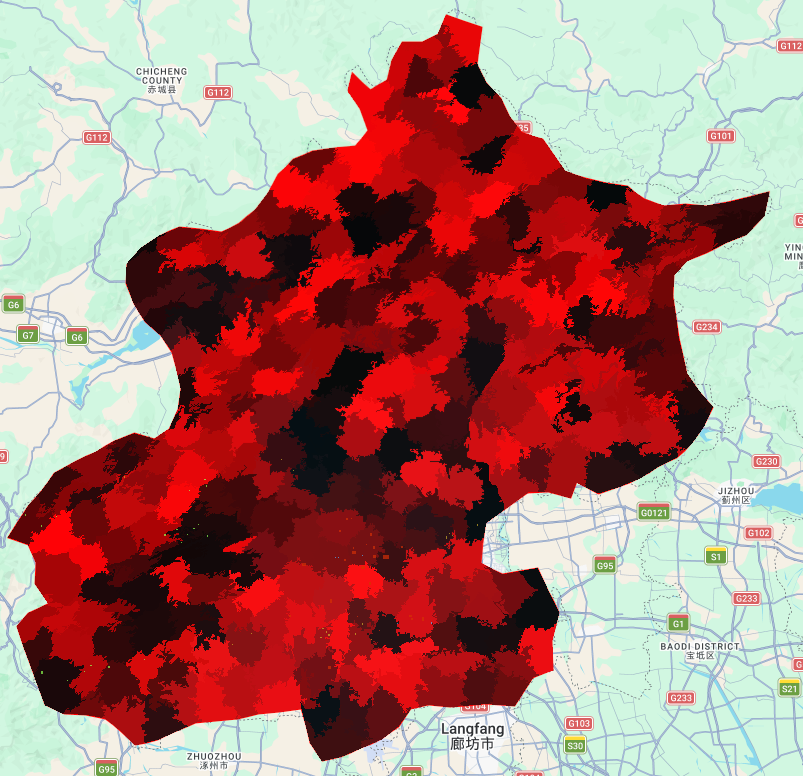
\includegraphics[width=1\linewidth,height=\textheight,keepaspectratio]{images/clipboard-2859904163.png}

}

\caption{Sub-pixel Fractional Abundance Map}

\end{figure}%

\begin{figure}[H]

{\centering 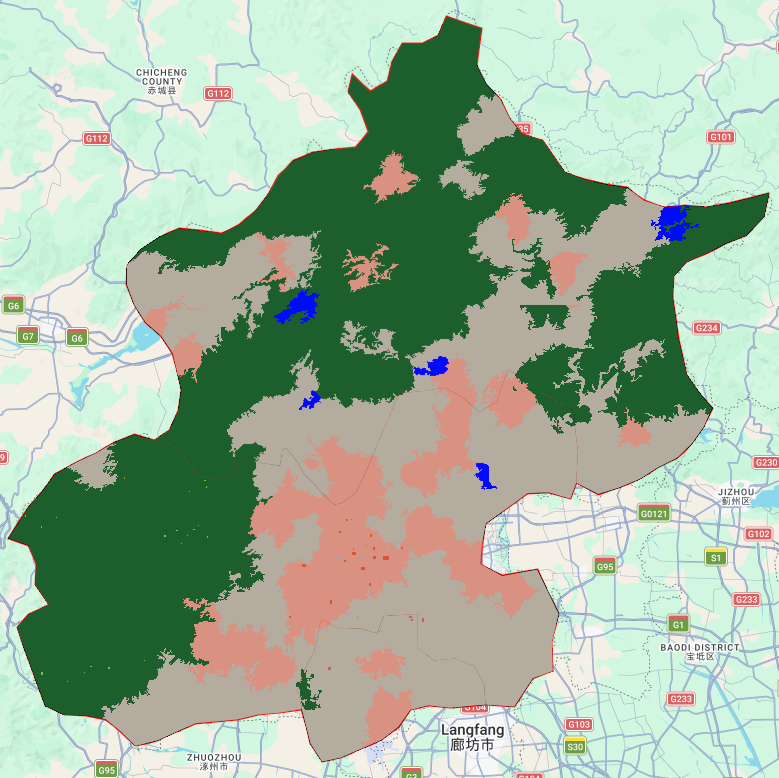
\includegraphics[width=0.93\linewidth,height=\textheight,keepaspectratio]{images/clipboard-2072705216.png}

}

\caption{Hardened Classification Map}

\end{figure}%

\section{Application}\label{application-3}

Traditional single-label classification often struggles with
medium-resolution imagery, for example, Landsat. However, studies like
(Wu 2004) ingeniously applied sub-pixel unmixing via the
vegetation--impervious surface--soil (V--I--S) model model. By
quantifying the proportions of these components within each pixel, this
technique effectively addresses the ``gray zone'' problem in highly
mixed urban centers, providing precise abundance indicators for
macro-level urban expansion and heat island assessments.

However, as very high-resolution imagery becomes more common, the main
challenge shifts from mixed pixels to the ``salt-and-pepper'' effect.
(Myint et al. 2011)show that object-based methods can handle this
problem much more effectively. By grouping neighbouring pixels into
larger areas with similar patterns, this approach can distinguish
between surfaces that look similar in colour but differ in structure,
like separating textured building roofs from smoother concrete spaces.

\begin{figure}[H]

{\centering 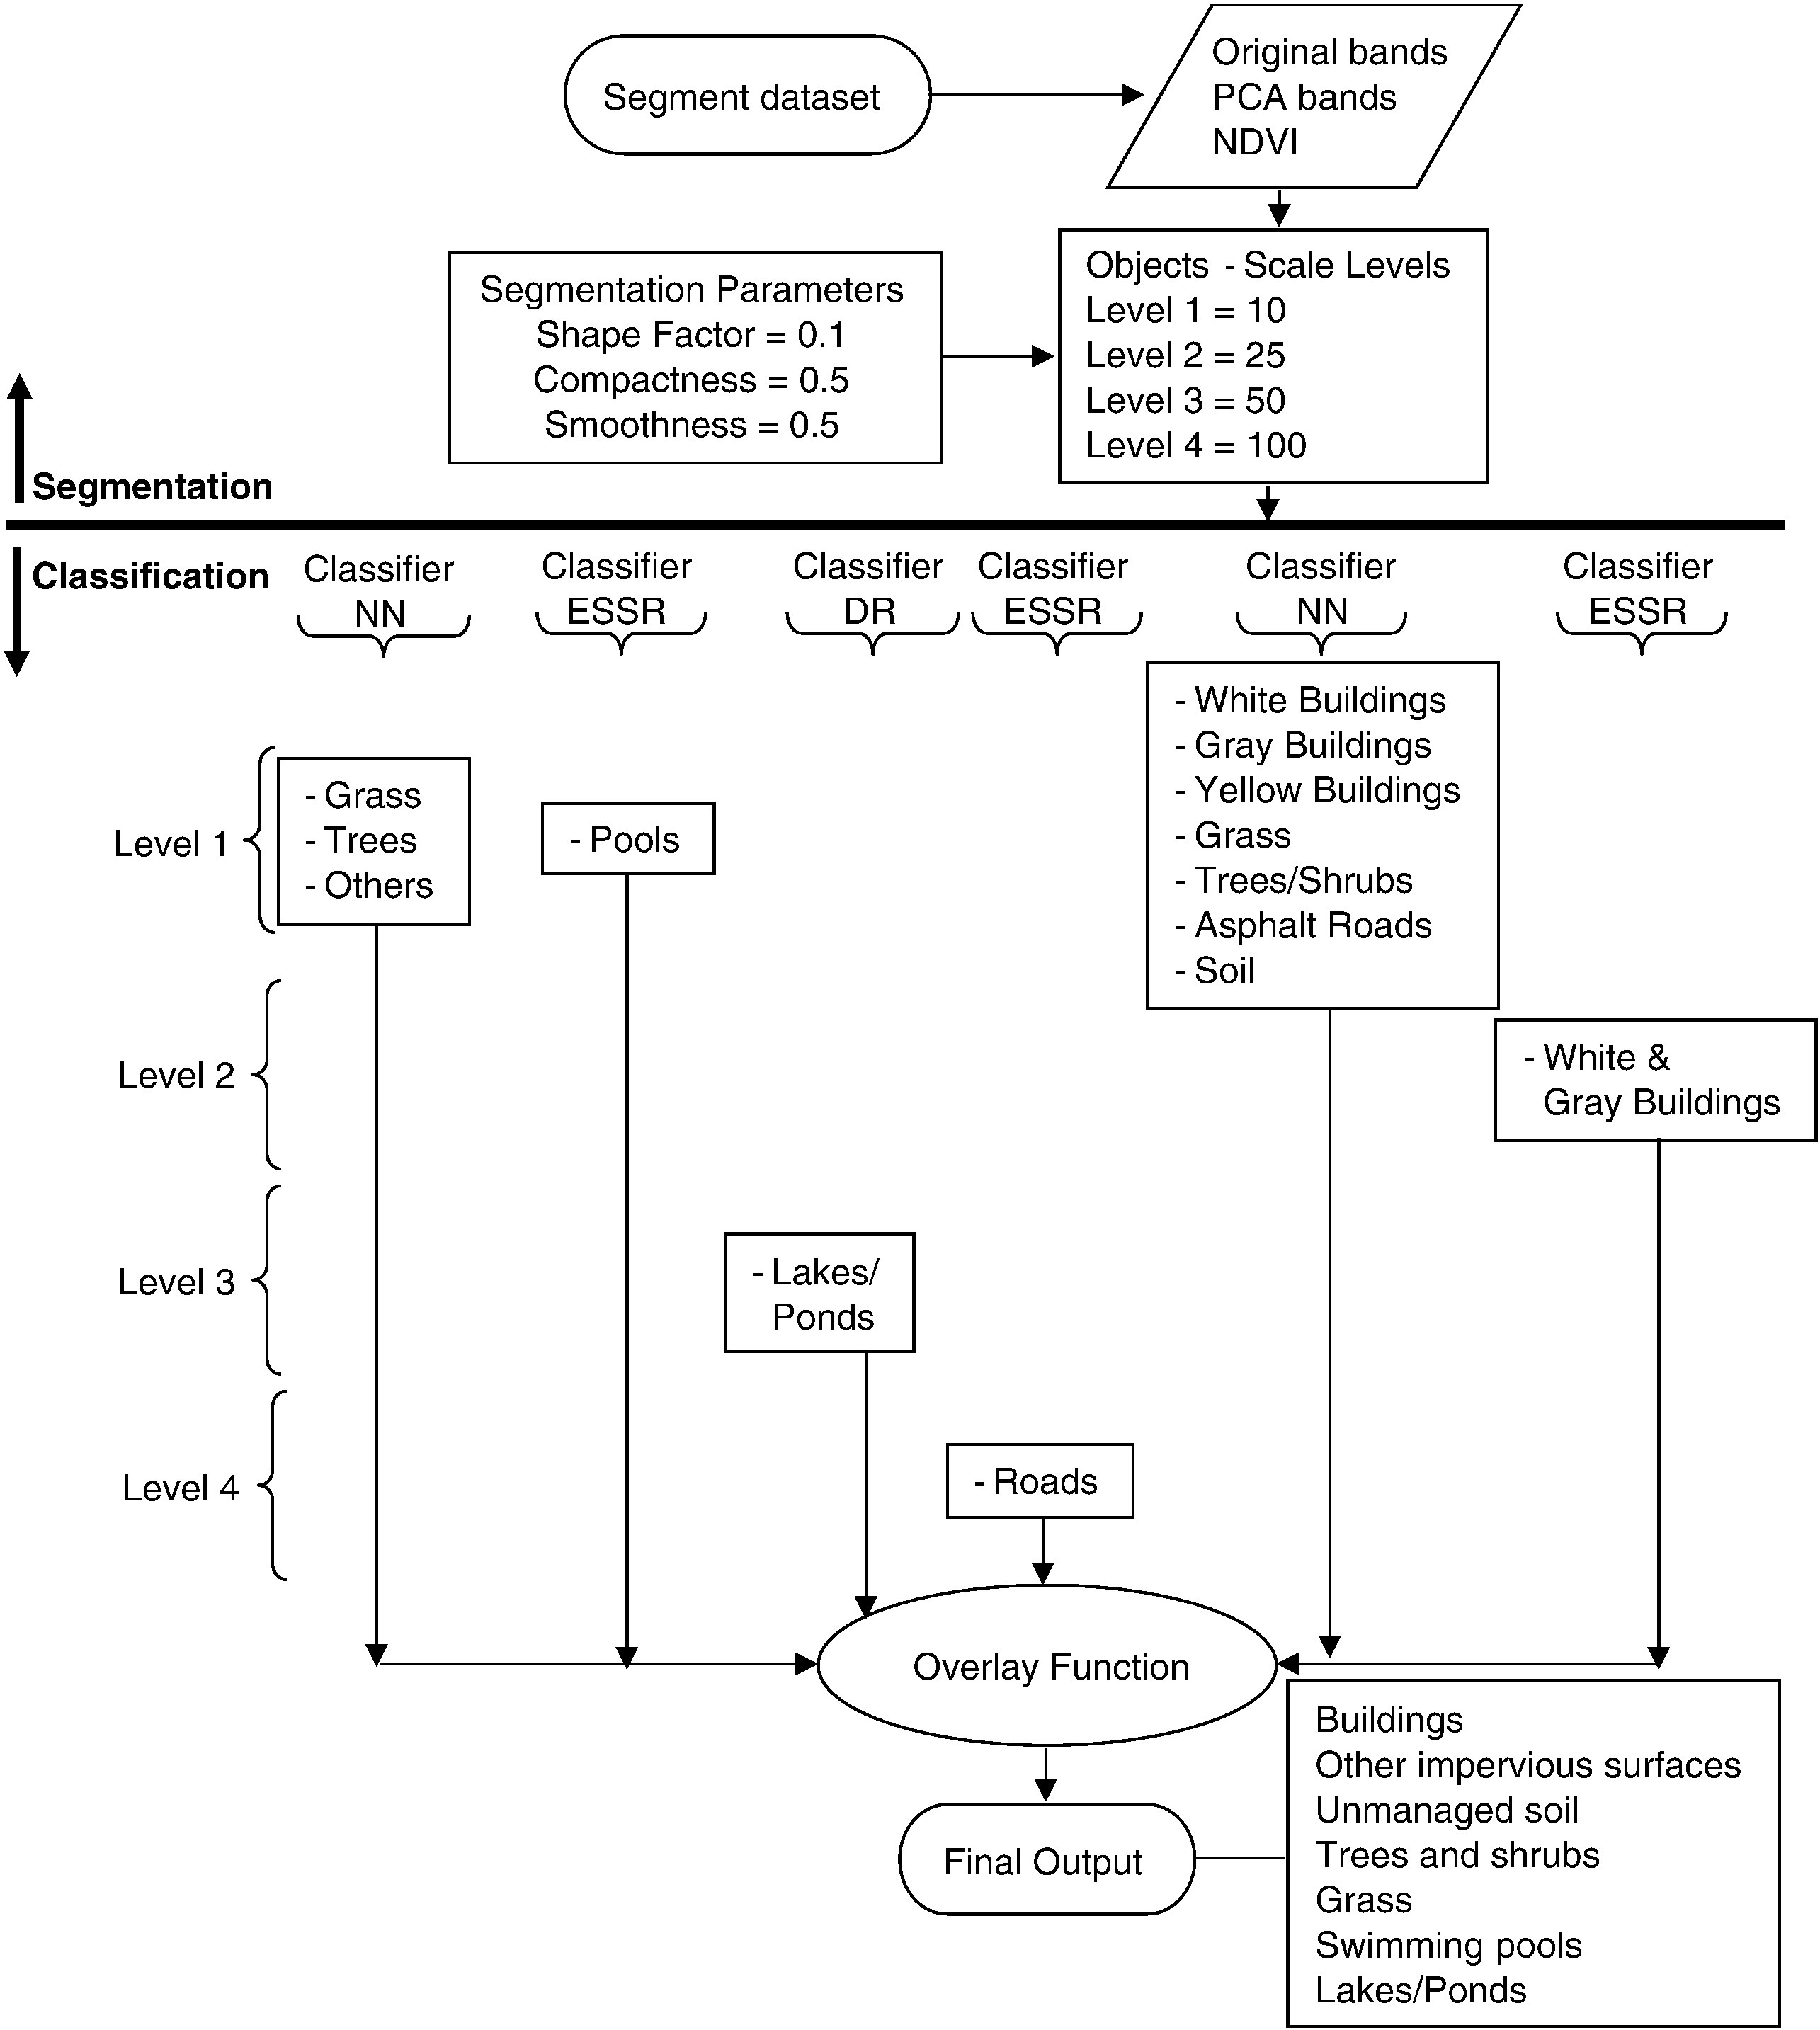
\includegraphics[width=5.96875in,height=\textheight,keepaspectratio]{images/clipboard-1169381459.png}

}

\caption{A flow chart demonstrating the overall procedure to generate a
final output.(Myint et al. 2011)}

\end{figure}%

Although both methods are widely used in the literature, they still have
clear limitations. Sub-pixel approaches can provide detailed proportions
of different land cover types, but they lose information about how these
elements are actually arranged within a pixel. For example, a pixel
showing 50\% vegetation does not reveal whether this represents a single
large green space or many small, scattered trees, which limits its
usefulness for practical decision making.

On the other hand, object-based methods depend heavily on how the
segmentation is set up, which is often based on the researcher's own
judgement (Blaschke, 2010). When applied to highly varied environments
across larger areas, this approach can require repeated adjustment of
parameters. It is time consuming and difficult to apply consistently at
scale.

\begin{figure}[H]

{\centering 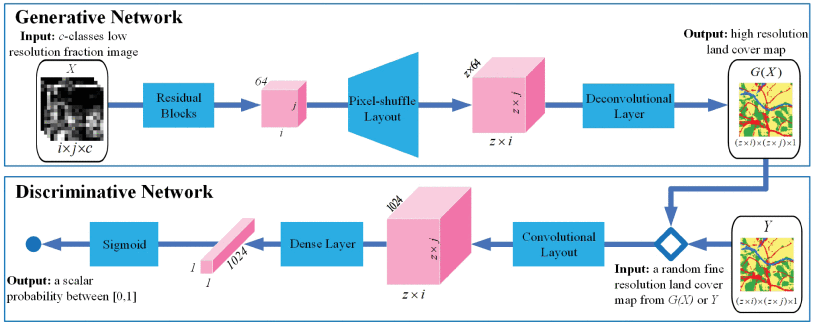
\includegraphics[width=6.72917in,height=\textheight,keepaspectratio]{images/clipboard-1946780496.png}

}

\caption{Architecture of the generative and discriminative networks of
the GAN-SRM.(Shang et al. 2022)}

\end{figure}%

Recent studies have begun to move beyond simply estimating land cover
proportions by introducing deep learning approaches for
higher-resolution mapping. For example, (Shang et al. 2022) applies a
generative adversarial network (GAN) to produce fine-scale land cover
maps from coarse imagery. Instead of only providing percentage
information within each pixel, this method generates a more detailed
spatial pattern, making the results more visually realistic and easier
to interpret.

\section{Reflection}\label{reflection-4}

While examining the intermediate SNIC outputs and the sub-pixel
proportion maps, I noticed that striping effects from Landsat scene
boundaries were quite visible. Reflecting on this, it seems that both
methods are highly sensitive to absolute spectral values, which means
that atmospheric differences between images from different dates or
orbital paths can be unintentionally amplified.

In addition, the relatively small number of training samples I used
around 20 polygons per class, may limited the model's ability to capture
more subtle variations in land cover. This suggests that, beyond the
choice of method or segmentation approach, the quality and diversity of
training data play a crucial role in determining the final results. A
more comprehensive and representative training dataset would likely
improve the model's performance, especially in complex urban
environments.

In short, choosing the right method involves trade-offs between detail
and spatial coherence, and the optimal choice may vary depending on the
complexity of the urban environment and the scale of the mapping
project.

\bookmarksetup{startatroot}

\chapter{Temperature}\label{temperature}

\section{Summary}\label{summary-4}

This week focused on understanding land surface temperature (LST)
derived from remote sensing data. A key takeaway is that satellites such
as Landsat can measure emitted radiation from the Earth's surface, which
can then be converted into temperature using radiative transfer
equations. The process involves several steps including converting
digital numbers (DN) to radiance, then to brightness temperature, and
finally adjusting for emissivity to obtain land surface temperature.

\phantomsection\label{fancy-layout}
\phantomsection\label{first-pic}
\begin{figure}[H]

{\centering 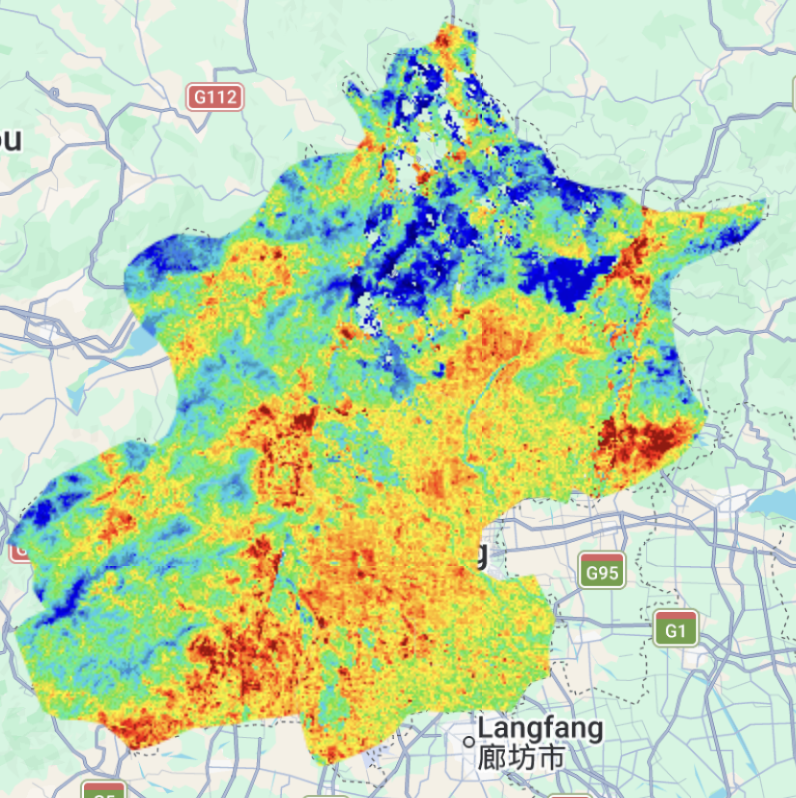
\includegraphics[width=1\linewidth,height=\textheight,keepaspectratio]{images/clipboard-1385091832.png}

}

\caption{Mean Landsat LST for Beijing in 2023}

\end{figure}%

\phantomsection\label{second-pic}
\begin{figure}[H]

{\centering 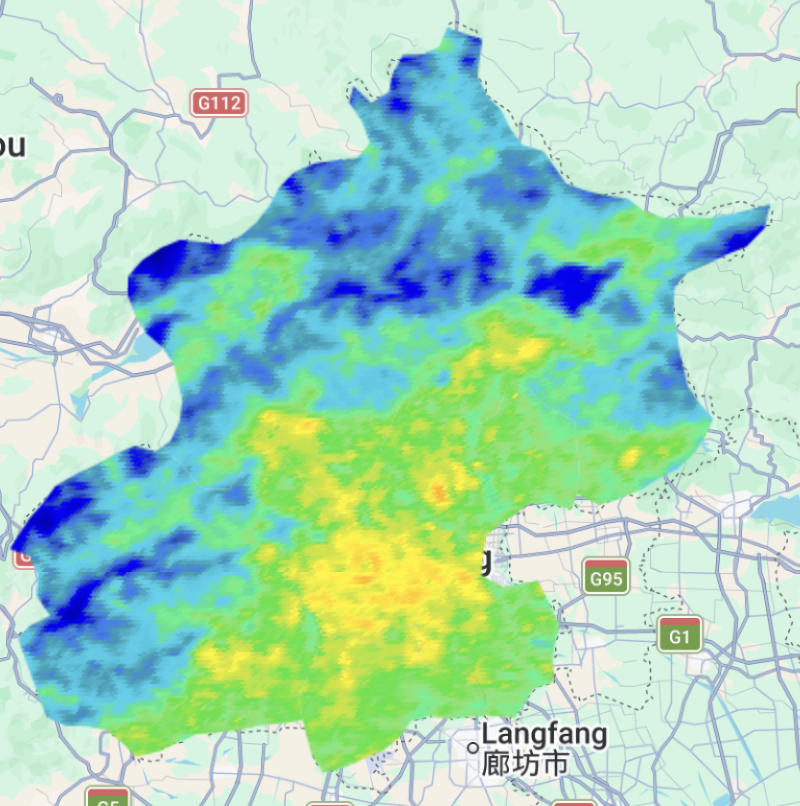
\includegraphics[width=0.99\linewidth,height=\textheight,keepaspectratio]{images/clipboard-1027079445.png}

}

\caption{Mean MODIS LST for Beijing in 2023}

\end{figure}%

\textbf{Comparison of Key Satellite Sensors for Land Surface
Temperature}

\begin{longtable}[]{@{}
  >{\raggedright\arraybackslash}p{(\linewidth - 6\tabcolsep) * \real{0.1421}}
  >{\raggedright\arraybackslash}p{(\linewidth - 6\tabcolsep) * \real{0.1148}}
  >{\raggedright\arraybackslash}p{(\linewidth - 6\tabcolsep) * \real{0.1366}}
  >{\raggedright\arraybackslash}p{(\linewidth - 6\tabcolsep) * \real{0.5956}}@{}}
\toprule\noalign{}
\begin{minipage}[b]{\linewidth}\raggedright
Satellite / Sensor Name
\end{minipage} & \begin{minipage}[b]{\linewidth}\raggedright
Spatial Resolution
\end{minipage} & \begin{minipage}[b]{\linewidth}\raggedright
Temporal Resolution
\end{minipage} & \begin{minipage}[b]{\linewidth}\raggedright
Key Features \& Applications
\end{minipage} \\
\midrule\noalign{}
\endhead
\bottomrule\noalign{}
\endlastfoot
\textbf{Landsat 8/9 (TIRS)} & 100m & 16 days & \textbf{Features:} High
spatial detail, but lower chance of cloud-free images.

\textbf{Applications:} Neighborhood-scale UHI assessment, microclimate
\& green space cooling effects. \\
\textbf{Terra/Aqua (MODIS)} & 1000m & 1-2 times/day & \textbf{Features:}
High observation frequency, ideal for time-series, but coarse spatial
detail.

\textbf{Applications:} Large-scale, long-term LST monitoring, extreme
heatwave warnings. \\
\textbf{Suomi NPP (VIIRS)} & 750m & At least 1-2 times/day &
\textbf{Features:} Next-gen replacement for MODIS, wider swath,
excellent radiometric calibration.

\textbf{Applications:} Regional thermal environment monitoring, urban
composite analysis with nighttime lights. \\
\textbf{Sentinel-3 (SLSTR)} & 1000m & \textless{} 1 day &
\textbf{Features:} Unique dual-view observation, highly accurate LST
retrieval.

\textbf{Applications:} Large-scale climate modeling, high-precision
regional thermal dynamics. \\
\textbf{Terra (ASTER)} & 90m & 16 days & \textbf{Features:} Extreme
spatial resolution, but non-continuous global imaging.

\textbf{Applications:} High-precision historical LST retrieval for
specific small areas. \\
\end{longtable}

Most LST studies rely on Landsat imagery, especially Landsat 5 and 8,
and tend to focus on semi-arid, tropical, and temperate regions. In
polar areas, where cloud cover is frequent, researchers often use MODIS
for its wider coverage and higher temporal resolution(Mohamed,
Lorestani, and Shabani 2025).

\begin{figure}[H]

{\centering \includegraphics[width=6.42708in,height=\textheight,keepaspectratio]{images/clipboard-3929050240.png}

}

\caption{The Sankey diagram shows the relationship between countries,
climate zones, and satellite sensors used in Land Surface Temperature
(LST) and Land Use Land Cover (LULC) studies.(Naserikia et al. 2023)}

\end{figure}%

\section{Application}\label{application-4}

A lot of the literature this week focused on using LST to understand
urban heat patterns, especially the Urban Heat Island effect. More
recent studies seem to emphasise how strongly land use change affects
temperature. There are broader reviews suggesting that urbanisation
itself is one of the main drivers of increasing surface temperatures
globally(Mohamed, Lorestani, and Shabani 2025). However, despite strong
spatial correlations, these studies still rely on surface temperature
rather than air temperature, which may limit their direct applicability
to human thermal comfort(Naserikia et al. 2023). Human thermal comfort
depends on multiple factors such as air temperature, humidity and
radiation, and LST is not a direct measure of it.

\begin{figure}[H]

{\centering \includegraphics[width=6.42708in,height=\textheight,keepaspectratio]{images/clipboard-3801461519.png}

}

\caption{The temperature difference between LST and Ta on acquisition
dates in Netatmo stations across Sydney.(Naserikia et al. 2023)}

\end{figure}%

Recent studies have extended this approach by linking LST with social
and spatial inequalities. In Chicago, high-resolution downscaled LST
data revealed significant differences in heat exposure across ethnic and
socioeconomically diverse communities, showing that urban heat does not
affect all residents equally(Lee et al. 2024). Similarly, a spatial
regression analysis across four major East Asian cities demonstrated
that land use composition and metropolitan structure strongly influence
LST distribution, emphasizing the role of urban planning in shaping
thermal environments(Li et al. 2022). In conclusion, this shifts LST
from being purely a physical measurement to a tool for understanding
environmental justice issues.

\begin{figure}[H]

{\centering \includegraphics[width=6.42708in,height=\textheight,keepaspectratio]{images/clipboard-3112875906.png}

}

\caption{Ethnic map of Humboldt Park region.(Lee et al. 2024)}

\end{figure}%

\section{Reflection}\label{reflection-5}

This week's content really opened my eyes. It did a great job connecting
abstract remote sensing data with real-world social issues. Looking at
these skills in the bigger context of urban planning, I not only learned
how to process temperature data and do zonal statistics in GEE, but also
started to see how remote sensing can actually be used as a powerful
tool to measure social inequality and support more sustainable city
planning.

For what comes next, since we can already use MODIS to track time-series
data and calculate average heat risk in specific areas, I think a really
interesting direction would be to combine dynamic LST data with more
detailed census data. That kind of spatial overlay could help us better
understand social vulnerability. And if we bring in methods like
geographically weighted regression, we could even figure out how
different environmental and social factors contribute to local
temperature differences. That would make it easier to design more
targeted strategies for climate adaptation.

\bookmarksetup{startatroot}

\chapter*{References}\label{references}
\addcontentsline{toc}{chapter}{References}

\markboth{References}{References}

\phantomsection\label{refs}
\begin{CSLReferences}{1}{0}
\bibitem[\citeproctext]{ref-Breiman2001RandomF}
Breiman, L. 2001. {``Random Forests.''} \emph{Machine Learning} 45:
5--32. \url{https://api.semanticscholar.org/CorpusID:89141}.

\bibitem[\citeproctext]{ref-breiman1984classification}
Breiman, Leo, Jerome Friedman, Richard A Olshen, and Charles J Stone.
1984. \emph{Classification and Regression Trees}. 1st ed. New York:
Chapman; Hall/CRC. \url{https://doi.org/10.1201/9781315139470}.

\bibitem[\citeproctext]{ref-rs16224287}
Cao, Cong-Yin, Meng-Ting Li, Yang-Jun Deng, Longfei Ren, Yi Liu, and
Xing-Hui Zhu. 2024. {``Joint Sparse Local Linear Discriminant Analysis
for Feature Dimensionality Reduction of Hyperspectral Images.''}
\emph{Remote Sensing} 16 (22). \url{https://doi.org/10.3390/rs16224287}.

\bibitem[\citeproctext]{ref-https:ux2fux2fdoi.orgux2f10.1155ux2f2018ux2f7973519}
Hess, Jeremy J., Sathish LM, Kim Knowlton, Shubhayu Saha, Priya Dutta,
Parthasarathi Ganguly, Abhiyant Tiwari, et al. 2018. {``Building
Resilience to Climate Change: Pilot Evaluation of the Impact of India's
First Heat Action Plan on All-Cause Mortality.''} \emph{Journal of
Environmental and Public Health} 2018 (1): 7973519.
https://doi.org/\url{https://doi.org/10.1155/2018/7973519}.

\bibitem[\citeproctext]{ref-su172210324}
Jocea, Andreea Florina, Liviu Porumb, Lucian Necula, and Dan Raducanu.
2025. {``Sentinel-2 Land Cover Classification: State-of-the-Art Methods
and the Reality of Operational Deployment---a Systematic Review.''}
\emph{Sustainability} 17 (22).
\url{https://doi.org/10.3390/su172210324}.

\bibitem[\citeproctext]{ref-rs16091639}
Lee, Jangho, Max Berkelhammer, Matthew D. Wilson, Natalie Love, and
Ralph Cintron. 2024. {``Urban Land Surface Temperature Downscaling in
Chicago: Addressing Ethnic Inequality and Gentrification.''}
\emph{Remote Sensing} 16 (9). \url{https://doi.org/10.3390/rs16091639}.

\bibitem[\citeproctext]{ref-li2022modeling}
Li, D., G. D. Newman, B. Wilson, Y. Zhang, and R. D. Brown. 2022.
{``Modeling the Relationships Between Historical Redlining, Urban Heat,
and Heat-Related Emergency Department Visits: An Examination of 11 Texas
Cities.''} \emph{Environment and Planning B: Urban Analytics and City
Science} 49 (3): 933--52.
\url{https://doi.org/10.1177/23998083211039854}.

\bibitem[\citeproctext]{ref-MOHAMED2025100315}
Mohamed, Ali, Niloufar Lorestani, and Farzin Shabani. 2025. {``Impact of
Urbanization on Land Surface Temperature: A Global Perspective.''}
\emph{Current Research in Environmental Sustainability} 10: 100315.
https://doi.org/\url{https://doi.org/10.1016/j.crsust.2025.100315}.

\bibitem[\citeproctext]{ref-s19173701}
Mohammad, Pir, Ajanta Goswami, and Stefania Bonafoni. 2019. {``The
Impact of the Land Cover Dynamics on Surface Urban Heat Island
Variations in Semi-Arid Cities: A Case Study in Ahmedabad City, India,
Using Multi-Sensor/Source Data.''} \emph{Sensors} 19 (17).
\url{https://doi.org/10.3390/s19173701}.

\bibitem[\citeproctext]{ref-MYINT20111145}
Myint, Soe W., Patricia Gober, Anthony Brazel, Susanne Grossman-Clarke,
and Qihao Weng. 2011. {``Per-Pixel Vs. Object-Based Classification of
Urban Land Cover Extraction Using High Spatial Resolution Imagery.''}
\emph{Remote Sensing of Environment} 115 (5): 1145--61.
https://doi.org/\url{https://doi.org/10.1016/j.rse.2010.12.017}.

\bibitem[\citeproctext]{ref-NASERIKIA2023167306}
Naserikia, Marzie, Melissa A. Hart, Negin Nazarian, Benjamin Bechtel,
Mathew Lipson, and Kerry A. Nice. 2023. {``Land Surface and Air
Temperature Dynamics: The Role of Urban Form and Seasonality.''}
\emph{Science of The Total Environment} 905: 167306.
https://doi.org/\url{https://doi.org/10.1016/j.scitotenv.2023.167306}.

\bibitem[\citeproctext]{ref-PENG2020106671}
Peng, Kaifeng, Weiguo Jiang, Yue Deng, Yinghui Liu, Zhifeng Wu, and
Zheng Chen. 2020. {``Simulating Wetland Changes Under Different
Scenarios Based on Integrating the Random Forest and CLUE-s Models: A
Case Study of Wuhan Urban Agglomeration.''} \emph{Ecological Indicators}
117: 106671.
https://doi.org/\url{https://doi.org/10.1016/j.ecolind.2020.106671}.

\bibitem[\citeproctext]{ref-8736016}
Roy, Swalpa Kumar, Gopal Krishna, Shiv Ram Dubey, and Bidyut B.
Chaudhuri. 2020. {``HybridSN: Exploring 3-d--2-d CNN Feature Hierarchy
for Hyperspectral Image Classification.''} \emph{IEEE Geoscience and
Remote Sensing Letters} 17 (2): 277--81.
\url{https://doi.org/10.1109/LGRS.2019.2918719}.

\bibitem[\citeproctext]{ref-Sabaghy2025}
Sabaghy, Sabah, Mohammad Abuzar, Doug Crawford, Andy McAllister, and
Kathryn Sheffield. 2025. {``Remote Sensing for Land Cover Mapping Across
Victoria, Australia -- a Machine Learning Application.''}
\emph{Scientific Data} 12 (1): 566.
\url{https://doi.org/10.1038/s41597-025-04900-5}.

\bibitem[\citeproctext]{ref-9195742}
Shang, Cheng, Xiaodong Li, Giles M. Foody, Yun Du, and Feng Ling. 2022.
{``Superresolution Land Cover Mapping Using a Generative Adversarial
Network.''} \emph{IEEE Geoscience and Remote Sensing Letters} 19: 1--5.
\url{https://doi.org/10.1109/LGRS.2020.3020395}.

\bibitem[\citeproctext]{ref-SHARMA2024101832}
Sharma, Ayushi, Priya Dutta, Priyanka Shah, Veena Iyer, Hao He, Amir
Sapkota, Chuansi Gao, and Yu-Chun Wang. 2024. {``Characterizing the
Effects of Extreme Heat Events on All-Cause Mortality: A Case Study in
Ahmedabad City of India, 2002--2018.''} \emph{Urban Climate} 54: 101832.
https://doi.org/\url{https://doi.org/10.1016/j.uclim.2024.101832}.

\bibitem[\citeproctext]{ref-10183518}
Sharma, Srashti, Aashutosh Singh, Rahul Kumar, and Anand Mehta. 2023.
{``Analysis of Land Surface Temperature at 10-Meter Pixel Size (Spatial
Resolution) for Ahmedabad City.''} In \emph{2023 International
Conference on Computational Intelligence and Sustainable Engineering
Solutions (CISES)}, 134--38.
\url{https://doi.org/10.1109/CISES58720.2023.10183518}.

\bibitem[\citeproctext]{ref-rs13234927}
Wang, Zhao, Fenlong Jiang, Tongfei Liu, Fei Xie, and Peng Li. 2021.
{``Attention-Based Spatial and Spectral Network with PCA-Guided
Self-Supervised Feature Extraction for Change Detection in Hyperspectral
Images.''} \emph{Remote Sensing} 13 (23).
\url{https://doi.org/10.3390/rs13234927}.

\bibitem[\citeproctext]{ref-WU2004480}
Wu, Changshan. 2004. {``Normalized Spectral Mixture Analysis for
Monitoring Urban Composition Using ETM+ Imagery.''} \emph{Remote Sensing
of Environment} 93 (4): 480--92.
https://doi.org/\url{https://doi.org/10.1016/j.rse.2004.08.003}.

\bibitem[\citeproctext]{ref-ZABALZA2014112}
Zabalza, Jaime, Jinchang Ren, Mingqiang Yang, Yi Zhang, Jun Wang,
Stephen Marshall, and Junwei Han. 2014. {``Novel Folded-PCA for Improved
Feature Extraction and Data Reduction with Hyperspectral Imaging and SAR
in Remote Sensing.''} \emph{ISPRS Journal of Photogrammetry and Remote
Sensing} 93: 112--22.
https://doi.org/\url{https://doi.org/10.1016/j.isprsjprs.2014.04.006}.

\end{CSLReferences}




\end{document}
